\documentclass[11pt,a4paper]{article}

% ATS-friendly / clean text extraction, matching the repository convention.
\input{glyphtounicode}
\pdfgentounicode=1
% glyphtounicode.tex does not map the large cmex/lmex operators, so summation and radical
% signs are lost on text extraction unless they are mapped here by hand.
\pdfglyphtounicode{summationdisplay}{2211}
\pdfglyphtounicode{summationtext}{2211}
\pdfglyphtounicode{radicalbig}{221A}
\pdfglyphtounicode{radical}{221A}

\usepackage[T1]{fontenc}
\usepackage[utf8]{inputenc}
\usepackage{lmodern}
\usepackage[margin=2.2cm]{geometry}
\usepackage{amsmath}
\usepackage{amssymb}
\usepackage{graphicx}
\usepackage{siunitx}
\usepackage{array}
\usepackage{booktabs}
\newcolumntype{L}[1]{>{\raggedright\arraybackslash}p{#1}}
\usepackage{caption}
\usepackage{subcaption}
\usepackage{float}
\usepackage{microtype}
\usepackage{fancyhdr}
\usepackage{xcolor}
\usepackage{mdframed}
\usepackage[hidelinks]{hyperref}
\hypersetup{%
  pdftitle={Electron Spin Resonance and Nuclear Magnetic Resonance},
  pdfauthor={Abdullah Alkabbawi},
  pdfsubject={Representative data. Not a record of measured results.},
}

\sisetup{separate-uncertainty=true, range-phrase={ to }, range-units=single}
\DeclareSIUnit{\gauss}{G}

\captionsetup{font=footnotesize,labelfont=bf,width=0.95\textwidth,skip=5pt}
\setlength{\parskip}{1pt}
\setlength{\floatsep}{8pt plus 2pt minus 2pt}
\setlength{\textfloatsep}{9pt plus 2pt minus 2pt}
\setlength{\intextsep}{8pt plus 2pt minus 2pt}
\renewcommand{\topfraction}{0.94}
\renewcommand{\bottomfraction}{0.80}
\renewcommand{\textfraction}{0.05}
\renewcommand{\floatpagefraction}{0.85}
\setlength{\abovedisplayskip}{5pt plus 2pt minus 2pt}
\setlength{\belowdisplayskip}{5pt plus 2pt minus 2pt}
\makeatletter
\renewcommand\section{\@startsection{section}{1}{\z@}%
  {-2.2ex \@plus -0.8ex \@minus -.2ex}{1.1ex \@plus .2ex}{\normalfont\large\bfseries}}
\renewcommand\subsection{\@startsection{subsection}{2}{\z@}%
  {-1.9ex \@plus -0.8ex \@minus -.2ex}{0.7ex \@plus .2ex}{\normalfont\normalsize\bfseries}}
\makeatother

\pagestyle{fancy}
\fancyhf{}
\fancyfoot[L]{\footnotesize Representative data. Not a record of measured results.}
\fancyfoot[R]{\footnotesize\thepage}
\renewcommand{\headrulewidth}{0pt}
\renewcommand{\footrulewidth}{0.4pt}
\fancypagestyle{plain}{%
  \fancyhf{}%
  \fancyfoot[L]{\footnotesize Representative data. Not a record of measured results.}%
  \fancyfoot[R]{\footnotesize\thepage}%
  \renewcommand{\headrulewidth}{0pt}%
  \renewcommand{\footrulewidth}{0.4pt}%
}

\title{\vspace{-1.2cm}\textbf{Electron Spin Resonance and Nuclear Magnetic Resonance}}
\author{Abdullah Alkabbawi\\[2pt]
\normalsize Physics 3H Laboratory (PHYS4009), School of Physics and Astronomy,\\
\normalsize University of Glasgow}
\date{\normalsize Session 2023-24}

\begin{document}

\maketitle
\thispagestyle{fancy}

\begin{abstract}
\noindent
The values reported here are representative data, generated to demonstrate the analysis. They are
not a record of measurements taken by the author. See the note immediately below.

\smallskip\noindent
Electron spin resonance (ESR) and nuclear magnetic resonance (NMR) were used to measure the
magnetic moments of an unpaired electron and of two spin one-half nuclei. A Helmholtz pair was
calibrated against a Hall magnetometer and gave a coil constant of
\SI{4.2073 \pm 0.0084}{\milli\tesla\per\ampere} (statistical;
\SI{\pm 0.043}{\milli\tesla\per\ampere} once the \SI{1}{\percent} field standard is included),
which is \SI{0.57}{\percent} below the value of
\SI{4.2314}{\milli\tesla\per\ampere} predicted by the Helmholtz formula for 320 turns per coil.
Resonance in solid DPPH was located at 24 frequencies between \SI{15}{\mega\hertz} and
\SI{130}{\mega\hertz}. The resonance frequency was linear in field with a gradient of frequency
against field of \SI{27.963 \pm 0.071}{\mega\hertz\per\milli\tesla} (statistical, with the
coil-constant calibration included), giving an electron spin g-factor of
$g_s = 1.998 \pm 0.005\,\text{(stat)} \pm 0.020\,\text{(syst)} = 1.998 \pm 0.021$. This is
\SI{0.22}{\percent} below the free-electron value $g_e = 2.0023$ and \SI{0.29}{\percent} below the
accepted solid-DPPH value $2.0036 \pm 0.0002$, an agreement at the level of 0.22 and 0.28
standard deviations respectively. The absorption line was
\SI{0.238 \pm 0.018}{\milli\tesla} wide at half
maximum, implying a transverse relaxation time of \SI{47.8 \pm 3.6}{\nano\second}, against
\SIrange{22}{44}{\nano\second} implied by the published peak-to-peak widths. An iron-cored
electromagnet was calibrated over
\SIrange{3.0}{4.0}{\ampere}; its gradient fell by \SI{20.6}{\percent} across that range and the
rising and falling branches differed by \SI{5.2}{\milli\tesla} at \SI{3.00}{\ampere}. Proton
resonance in glycerine gave a gradient of frequency against field of
\SI{42.48 \pm 0.38}{\mega\hertz\per\tesla} and $g(^{1}\mathrm{H}) = 5.57 \pm 0.08$, against a
literature value of $5.5857$ (0.17 standard deviations). Fluorine resonance in PTFE gave
\SI{39.56 \pm 0.69}{\mega\hertz\per\tesla} and $g(^{19}\mathrm{F}) = 5.19 \pm 0.10$, against
$5.2577$ (0.66 standard deviations). Polythene was found to resonate at
\SI{17.80 \pm 0.05}{\mega\hertz} at
\SI{0.4194}{\tesla}, which is about 0.3 standard deviations from the proton prediction and about
5 standard deviations from the
fluorine prediction once the \SI{1}{\percent} uncertainty on the calibrated field is carried,
identifying it as a hydrocarbon containing no fluorine.
\end{abstract}

\begin{mdframed}[backgroundcolor=gray!12, linecolor=gray!60, linewidth=0.8pt,
                 innertopmargin=8pt, innerbottommargin=8pt, innerleftmargin=10pt,
                 innerrightmargin=10pt, roundcorner=2pt]
\textbf{Note on the data in this report.}\\[2pt]
The original laboratory notebook for this experiment is no longer available. Every measured value
in this report, and every table and figure derived from measurements, is therefore
\textbf{representative}: they were generated
from accepted physical constants plus realistic instrument scatter, in order to demonstrate the
analysis, the uncertainty treatment and the physics of the experiment. \textbf{None of it is a
record of measurements taken by the author.} The apparatus, the procedure, the theory and the
literature comparisons are genuine and follow the departmental experiment information script.
The measurements themselves are not. Nothing in this document should be read, cited or reused as
experimental evidence.
\end{mdframed}

\section{Introduction}

Magnetic resonance is the absorption of electromagnetic radiation by a magnetic moment placed in
a static magnetic field. The moment has a set of discrete energy levels whose spacing is
proportional to the field, and when an applied photon matches that spacing, transitions are
driven and energy is absorbed. The absorption is sharp in frequency, so the field at which it
occurs can be located precisely, which is what makes the effect useful as a measurement.

Two versions of the same physics are studied here. In electron spin resonance (ESR), also called
electron paramagnetic resonance, the moment belongs to an unpaired electron. In nuclear magnetic
resonance (NMR) it belongs to an atomic nucleus. The two differ only in the size of the moment.
The nuclear magneton is smaller than the Bohr magneton by the ratio of the proton mass to the
electron mass, about 1836, but the proton g-factor is 5.586 against 2.002 for the electron, so
the resonance field needed at a given frequency is larger by $g_s\mu_B/(g_p\mu_n) = 658$, not by
1836 \cite{codata}. That single number explains almost every difference
between the two halves of the apparatus: ESR here uses air-cored Helmholtz coils producing a few
millitesla, while NMR needs an iron-cored electromagnet producing about \SI{0.42}{\tesla}.

Both techniques matter practically. ESR is limited to species with a permanent electronic
magnetic moment, so it is used on free radicals, transition-metal ions, colour centres and
conduction electrons, and the measured g-factor reports directly on the orbital environment of
the unpaired electron \cite{weilbolton}. NMR determines molecular structure and bonding across
chemistry and materials science, and is the physical basis of magnetic resonance imaging
\cite{abragam,slichter}. The organic free radical 2,2-diphenyl-1-picrylhydrazyl, referred to
throughout by its script name diphenyl-picryl-hydrazyl (DPPH), is used for the ESR half: it is
stable indefinitely as a solid at room temperature, carries one unpaired electron per molecule
and gives a single narrow line, which is why it is the standard ESR reference material
\cite{krzystek}. The NMR half uses glycerine and polystyrene as sources of protons, PTFE as a
source of fluorine, and polythene as an unknown to be identified from its resonance frequency.

The experiment has six objectives, taken from the departmental script \cite{script}. For ESR:
graph the resonance frequency as a function of magnetic field; determine the g-factor of DPPH;
and determine the line width of the resonance signal. For NMR: investigate the resonance of
protons in glycerine and polystyrene; investigate the resonance of fluorine in PTFE; and determine
the g-factors of the proton and of fluorine. The script also asks for the composition of polythene
to be deduced from its resonance frequency, and for the transients known as wiggles to be observed
and explained.

\section{Theory}

\subsection{Magnetic moments and the two magnetons}

An electron of charge $-e$ and mass $m_e$ moving in a circular orbit of radius $\rho$ at speed $v$
is a current loop of current $i = -ev/2\pi\rho$, so its magnetic moment is
\begin{equation}
\mu_L = iA = -\frac{ev}{2\pi\rho}\,\pi\rho^{2} = -\frac{e}{2m_e}\,(m_e v\rho) = -\frac{e}{2m_e}L
= -\frac{e\hbar}{2m_e}\,m_\ell \equiv -\mu_B m_\ell ,
\qquad
\mu_B = \frac{e\hbar}{2m_e} ,
\label{eq:bohr}
\end{equation}
where $L = m_\ell\hbar$ is the orbital angular momentum and
$\mu_B = \SI{9.2740100657e-24}{\joule\per\tesla}$ is the Bohr magneton, the script's equation (2).
Orbital motion therefore has a g-factor of exactly 1. Spin does not: the Dirac equation gives
$g_s = 2$ for a point spin one-half particle, and quantum electrodynamic corrections raise this
slightly. The general relation covering both contributions is the script's equation (1),
\begin{equation}
\boldsymbol{\mu}_J = -g_J\,\mu_B\,\frac{\mathbf{J}}{\hbar} ,
\label{eq:muJ}
\end{equation}
where $\mathbf{J}$ is the total electronic angular momentum and $g_J$ is the Lande splitting
factor, given for a state of well-defined $L$, $S$ and $J$ by
$g_J = 1 + [J(J+1) + S(S+1) - L(L+1)]/[2J(J+1)]$. For a pure spin state, $L = 0$ and $J = S = 1/2$,
so $g_J = 2 = g_s$. This is the case identified in the script: for DPPH the orbital contribution
is quenched and only the spin need be considered.

For a nucleus the same construction applies with the proton mass in place of the electron mass,
giving the nuclear magneton $\mu_n = e\hbar/2m_p = \SI{5.0507837393e-27}{\joule\per\tesla}$, so
that $\mu_B/\mu_n = m_p/m_e = 1836.2$. The nuclear moment is written, following the script's
equation (8), as
\begin{equation}
\boldsymbol{\mu} = g\,\mu_n\,\frac{\mathbf{S}}{\hbar} ,
\end{equation}
where $\mathbf{S}$ is the nuclear spin and $g$ the nuclear g-factor.\footnote{The script uses $S$
for the nuclear spin quantum number and $k$ for its projection, where most of the literature uses
$I$ and $m_I$. The script's symbols are kept throughout this report. Both $\mathbf{S}$ and
$\mathbf{J}$ carry units of angular momentum, so both moment definitions divide by $\hbar$. The
symbol $k_B$ always means the Boltzmann constant.} Unlike the electronic case, $g$ for a composite nucleus cannot be
calculated from first principles. The proton has $g = 5.586$ and the neutron $g = -3.826$, and
those anomalous values were among the first clear indications that neither particle is elementary.

\subsection{Zeeman splitting and the resonance condition}

The potential energy of a magnetic moment in a field $\mathbf{B} = B_0\hat{z}$ is the script's
equation (3), $E = -\boldsymbol{\mu}\cdot\mathbf{B}$. Substituting equation~\eqref{eq:muJ} gives
$E = g_J\mu_B m_J B_0$, and for the free electron $m_J \to m_s = \pm 1/2$, which is the script's
equation (4),
\begin{equation}
E_{\pm} = \pm\tfrac{1}{2}\,g_s\,\mu_B\,B_0 , \qquad m_s = \pm\tfrac{1}{2} ,
\end{equation}
corresponding to the electron magnetic moment being antiparallel and parallel to the field
respectively, that is to the spin being parallel and antiparallel to it. Because the
moment carries a minus sign relative to the spin, the lower state is the one in which the moment
is parallel to $\mathbf{B}$. The splitting is $\Delta E = g_s\mu_B B_0$.

An oscillating field $B_1$ applied perpendicular to $B_0$ drives magnetic dipole transitions with
the selection rule $\Delta m_s = \pm 1$. Absorption occurs when the photon energy matches the
splitting, which is the script's equation (5):
\begin{equation}
h\nu = g_s\,\mu_B\,B_0 .
\label{eq:esrres}
\end{equation}
Rearranged for the quantity the experiment extracts from a graph,
\begin{equation}
\boxed{\;g_s = \frac{h}{\mu_B}\left(\frac{\mathrm{d}\nu}{\mathrm{d}B_0}\right)\;} ,
\qquad \frac{h}{\mu_B} = \SI{7.144774e-11}{\tesla\second} .
\label{eq:gwork}
\end{equation}
The whole of ESR objectives (i) and (ii) reduces to measuring that gradient. Note that the
estimator is the gradient and not a single pair of readings. A constant offset in the field, for
example from the Earth's field, shifts the intercept and leaves the gradient untouched, so taking
the gradient makes the result immune to it. This point is used in Sections~\ref{sec:esrfit} and
\ref{sec:unc}.

The nuclear case is algebraically identical. With $2S+1$ equally spaced levels
\begin{equation}
E_k = -g\,\mu_n B_0\,k , \qquad k = -S,\,-S+1,\,\ldots,\,+S ,
\end{equation}
which is the script's equation (9), the selection rule $\Delta k = \pm 1$ gives the script's
equation (11),
\begin{equation}
h\nu = \left|E_{k+1} - E_k\right| = g\,\mu_n B_0 ,
\qquad
\boxed{\;g = \frac{h}{\mu_n}\left(\frac{\mathrm{d}\nu}{\mathrm{d}B_0}\right)\;} ,
\qquad \frac{h}{\mu_n} = \SI{1.311889e-7}{\tesla\second} .
\label{eq:nmrres}
\end{equation}
Both $^{1}\mathrm{H}$ and $^{19}\mathrm{F}$ have $S = 1/2$, so both have exactly two levels and a
single resonance line. Equal level spacing is what makes the spectrum a single line rather than a
multiplet: every allowed step on the ladder has the same energy.

The accepted gradients follow directly from the constants. For the free electron,
$g_e\mu_B/h = \SI{28.0250}{\mega\hertz\per\milli\tesla}$; for DPPH at $g = 2.0036$,
\SI{28.0429}{\mega\hertz\per\milli\tesla}; for the proton,
$g_p\mu_n/h = \SI{42.577478}{\mega\hertz\per\tesla}$; and for $^{19}$F,
$g_F\mu_n/h = \SI{40.077583}{\mega\hertz\per\tesla}$ \cite{codata,stone,harris}.

\subsection{Why DPPH, and why the g-factor sits close to two}

Equation~\eqref{eq:esrres} describes something observable only if the sample has a non-zero
electronic magnetic moment in its ground state. In a closed-shell molecule every orbital is
doubly occupied with paired spins, the total electronic angular momentum vanishes, and there is
no splitting to detect. A paramagnetic species is one with a permanent non-zero total electronic
angular momentum, which in practice means an unpaired electron. DPPH is a stable free radical
whose unpaired electron sits on the hydrazyl bridge and is delocalised over the two hydrazyl
nitrogen atoms and out into the surrounding rings.

Two effects fix its g-factor. First, orbital quenching. DPPH is a low-symmetry organic molecule
with an orbitally non-degenerate ground state whose wavefunction can be taken real, and for a
real wavefunction $\langle\psi|\hat{L}_i|\psi\rangle = 0$, because $\hat{L}_i$ is purely imaginary
in the position representation while the expectation value of a Hermitian operator must be real.
Physically, the electron occupies a standing-wave molecular orbital held in place by the bonding
framework rather than a circulating one, so the orbital contribution is quenched to first order
and $g_J \to g_s \approx 2$.

Second, a small residual shift, because quenching is not complete. Spin-orbit coupling mixes a
little excited-state orbital character into the ground state, and second-order perturbation theory
gives
\begin{equation}
\Delta g_{ii} = g_{ii} - g_e = -2\lambda\,\Lambda_{ii} ,
\qquad
\Lambda_{ii} = \sum_{n \neq 0}
\frac{\left|\langle 0|\hat{L}_i|n\rangle\right|^{2}}{E_n - E_0} ,
\end{equation}
which is a tensor; a single principal component is quoted here. Every term of the sum is
positive, so the sign of $\Delta g_{ii}$ is the opposite of the sign of the effective spin-orbit
constant. The sign is positive for DPPH because the spin density sits on the hydrazyl nitrogens,
where the relevant excitations are from filled orbitals, so the effective spin-orbit constant is
negative and $\Delta g$ comes out positive.
For a light-atom organic radical the spin-orbit constant $\lambda$ is small in magnitude and the
relevant excitation energies are of order several electronvolts, so $\Delta g$ is only about
$+1.3\times10^{-3}$, giving $g(\mathrm{DPPH}) = 2.0036 \pm 0.0002$, about \SI{0.065}{\percent}
above $g_e$ \cite{krzystek}. That shift is a chemical fingerprint, and reading it is the whole
basis of ESR as a structural technique. Section~\ref{sec:disc} returns to whether the present
apparatus can resolve it.

\subsection{Population differences and signal strength}

The absorption signal exists only because the lower level is slightly more populated than the
upper one. The populations follow the script's equation (10), the Boltzmann distribution, and for
a two-level system the fractional excess in the lower level is
\begin{equation}
P = \frac{N_+ - N_-}{N_+ + N_-} = \tanh\!\left(\frac{\Delta E}{2k_B T}\right)
\simeq \frac{\Delta E}{2k_B T} ,
\end{equation}
the approximation being excellent because $\Delta E/k_B T \sim 10^{-6}$ here. At the laboratory
temperature of \SI{295}{\kelvin} recorded in Section~\ref{sec:apparatus}, DPPH at
$B_0 = \SI{2.0}{\milli\tesla}$ gives $P = \SI{4.6}{ppm}$, about five spins in a
million, and protons at \SI{0.43}{\tesla} give $P = \SI{1.49}{ppm}$.
Two comparisons follow and are used in the discussion. At equal field the
electron splitting exceeds the proton splitting by $g_s\mu_B/g_p\mu_n = 658.2$. For
induction-detected magnetic resonance the signal scales as $\gamma^{3}B_0^{2}$, because the
induced electromotive force carries an extra factor of the precession frequency, so at equal
field the electron advantage is $658.2^{3} = 2.85\times10^{8}$. That $\gamma^{3}B_0^{2}$ scaling
is the standard figure of merit for induction detection and is quoted here only for orientation.
The present rig detects the loss in a marginal oscillator rather than an induced electromotive
force, as Section~\ref{sec:marginal} describes, so its signal is proportional to
$\eta\chi''Q$ and carries an additional dependence on $T_2$; the exact power of $\gamma$ therefore
differs, though the order of magnitude of the advantage does not. A commercial X-band
spectrometer at
\SI{0.34}{\tesla} and the same temperature achieves $P = \SI{776}{ppm}$, a factor of 170 better
than the present rig.

\subsection{The Helmholtz field}

A single circular loop of radius $r$ carrying current $I$ produces an on-axis field
$B(z) = \mu_0 I r^{2}/[2(r^{2}+z^{2})^{3/2}]$ at axial distance $z$. Two identical coaxial coils of
$n$ turns each, separated by $d = r$, give at the midpoint
\begin{equation}
B_0 = 2\times\frac{\mu_0 n I r^{2}}{2\left(r^{2} + (r/2)^{2}\right)^{3/2}}
= \left(\frac{4}{5}\right)^{3/2}\frac{\mu_0\,n\,I}{r} ,
\label{eq:helm}
\end{equation}
which is the script's equation (6). The first derivative vanishes at the midpoint by symmetry for
any separation. The separation $d = r$ is chosen because it also makes the second derivative
vanish, and the third vanishes by symmetry, so the leading non-uniformity is fourth order,
leaving $B(z) = B_0[1 - (144/125)(z/r)^{4} + \ldots]$.
Over a \SI{6}{\milli\metre} sample at $r = \SI{68}{\milli\metre}$ the on-axis fractional variation
is only $4.36\times10^{-6}$, which is negligible.

Evaluating with $\mu_0 = 4\pi\times10^{-7}\,\si{\volt\second\per\ampere\per\metre}$, $n = 320$ and
$r = \SI{6.8}{\centi\metre}$ gives $(4/5)^{3/2} = 0.71554$,
$\mu_0 n/r = \SI{5.913586e-3}{\tesla\per\ampere}$ and therefore
$B_0 = \SI{4.2314}{\milli\tesla\per\ampere}\times I$. The script states this simplifies to
$B_0 = 4.23I$ in millitesla, which is confirmed to three significant figures. It nevertheless
instructs that the measured calibration be used in preference, since the coils may not have
exactly the stated number of turns. That instruction is followed here and
equation~\eqref{eq:helm} is used only as a comparison.

\subsection{Line width and relaxation}
\label{sec:theorywidth}

Following the script, $\Delta B_0$ denotes the \emph{full width at half maximum} (FWHM) of the
absorption line. The script calls this the half-width, but the procedure it prescribes measures the
width at half the full signal height, which is the FWHM. The distinction matters by a factor of two
in the relaxation time and by $\sqrt{3}$ in the comparison with published widths, so it is fixed
here and used consistently. For a homogeneously broadened line the absorption is Lorentzian,
$\chi''(\omega) \propto T_2/[1 + (\omega-\omega_0)^{2}T_2^{2}]$, whose half-width at half maximum
in angular frequency is $1/T_2$. Converting to field units through $\omega = \gamma B$ with
$\gamma = g\mu_B/\hbar$,
\begin{equation}
\Delta B_0^{\mathrm{FWHM}} = \frac{2}{\gamma T_2} = \frac{2\hbar}{g\mu_B T_2} ,
\qquad\Longrightarrow\qquad
T_2 = \frac{2\hbar}{g\,\mu_B\,\Delta B_0} .
\label{eq:t2}
\end{equation}
Commercial spectrometers use lock-in detection and record the first derivative of the absorption,
so the literature quotes the peak-to-peak derivative width $\Delta B_{pp}$. For a Lorentzian the
derivative extrema sit at $\pm\Gamma/\sqrt{3}$, where $\Gamma$ is the half-width at half maximum,
giving
\begin{equation}
\Delta B_{pp} = \frac{\Delta B_0^{\mathrm{FWHM}}}{\sqrt{3}} .
\label{eq:pp}
\end{equation}
This conversion is applied before any comparison with published values is made.

Several mechanisms broaden the DPPH line. A rigid lattice of dipoles at the spacing found in solid
DPPH would give a width of order \SI{4.3}{\milli\tesla}, and the unresolved hyperfine structure
from the two hydrazyl nitrogens would add of order \SI{1}{\milli\tesla}. The line observed in the
solid is far narrower than either, because Heisenberg exchange between neighbouring radicals
motionally averages the local dipolar field. The Anderson-Weiss result for exchange narrowing is
$\Delta B_{\mathrm{obs}} \sim (\Delta B_{\mathrm{dip}})^{2}/\Delta B_{\mathrm{ex}}$, and it also
predicts that the surviving line shape is Lorentzian with extended wings rather than Gaussian
\cite{anderson}. The same mechanism collapses the nitrogen hyperfine quintet seen in dilute
solution into the single line seen in the solid.

For the NMR samples the controlling parameters are the relaxation times: $T_1$ governs the recovery
of the longitudinal magnetisation and therefore how easily the transition saturates, $T_2$ governs
the loss of transverse phase coherence, and the observed decay time follows
$1/T_2^{*} = 1/T_2 + \gamma\,\Delta B_0^{\mathrm{sample}}$, which adds dephasing from
inhomogeneity of $B_0$ across the sample. In a liquid such as glycerine the molecules reorient far
faster than the dipolar dephasing time, so the proton-proton coupling averages towards zero and the
line is narrow. In a glass such as polystyrene, well below its glass transition, the backbone does
not move on the resonance timescale, the full rigid-lattice coupling survives, and the line is
broad.

\subsection{Transient oscillations after passage}
\label{sec:theorywiggles}

The script asks for the transients known as wiggles to be observed and explained. Work in a frame
rotating at the fixed radio frequency and let $t = 0$ be the instant the swept field passes exactly
through resonance. Transverse magnetisation created at that instant precesses freely while the
field continues to move, so the offset grows linearly,
$\Delta\omega(t) = \gamma(\mathrm{d}B/\mathrm{d}t)\,t$, the accumulated phase is quadratic, and
the detected in-phase component behaves as
\begin{equation}
\phi(t) = \tfrac{1}{2}\gamma\left(\frac{\mathrm{d}B}{\mathrm{d}t}\right)t^{2} ,
\qquad
S(t) \propto \exp\left(-t/T_2^{*}\right)\cos\!\left[\tfrac{1}{2}\gamma\left(\mathrm{d}B/\mathrm{d}t\right)t^{2}\right] ,
\end{equation}
a chirped, decaying oscillation whose successive maxima fall at
$t_n = \sqrt{4\pi n / \gamma|\mathrm{d}B/\mathrm{d}t|}$. The spacing therefore shrinks as
$\sqrt{n+1}-\sqrt{n}$: the wiggles crowd closer together as they die away, and they only ever
trail the resonance, never precede it, because they are the free decay of magnetisation created at
the moment of passage. The number of maxima that appear before the envelope has decayed is
\begin{equation}
N = \frac{\gamma\left(\mathrm{d}B/\mathrm{d}t\right)\left(T_2^{*}\right)^{2}}{4\pi} ,
\label{eq:wiggles}
\end{equation}
so \emph{one} countable wiggle requires $\gamma(\mathrm{d}B/\mathrm{d}t)(T_2^{*})^{2} > 4\pi$ and
$n$ of them require $n$ times that. For a Lorentzian line the decay time is
$T_2^{*} = 1/\pi\,\Delta\nu$, with $\Delta\nu$ the line width in frequency units. The modulation
used here was about \SI{2.4}{\milli\tesla} peak at \SI{28}{\hertz}, so
$\mathrm{d}B/\mathrm{d}t = \SI{0.42}{\tesla\per\second}$ at the zero crossing, and four to six
wiggles then need $T_2^{*}$ of order a millisecond, hence a line no more than a few hundred hertz
wide. Their presence is thus a direct qualitative proof that the magnet is homogeneous and the
sample properly centred, and their number is a rough measure of $T_2^{*}$. The counts observed
are compared with equation~\eqref{eq:wiggles} in Section~\ref{sec:samples} and
Figure~\ref{fig:displays}. The effect was seen in the first nuclear induction experiments
\cite{bloch} and analysed shortly afterwards \cite{jacobsohn}.

\section{Apparatus and method}
\label{sec:apparatus}

Both halves of the experiment were run on the open bench at the ambient laboratory temperature of
\SI{295}{\kelvin}, about \SI{22}{\celsius}. Nothing in either procedure is temperature controlled
and no sample was heated or cooled, so the temperature enters the calculations in only one place:
it sets the Boltzmann population difference that makes the absorption detectable at all. Every
population calculation in this report, for the electron and for the proton alike, uses this value.
It matters qualitatively in one further place, since it fixes where each polymer sample sits
relative to its own glass transition, which is what Section~\ref{sec:samples} uses to explain the
line widths.

\subsection{ESR apparatus}

The ESR assembly comprised an ESR basic unit carrying the radio-frequency oscillator, an ESR
control unit, a pair of Helmholtz coils and a two-channel oscilloscope. The whole assembly was
clamped as shown in Appendix 3 of the script, because mechanical instability spoils the sharpness
of the resonance by modulating the position of the sample in both the static field and the
radio-frequency coil.

The Helmholtz coils were positioned mechanically parallel at a separation of
\SI{6.8}{\centi\metre}, equal to the coil radius, since the separation fixes the field
configuration. They were connected electrically in series, the E and E sockets joined and the A
sockets taken to the current supply of the ESR control unit. The basic unit was connected to the
control unit through the six-pole cable at the socket labelled PROBE, the ESR SIGNAL output taken
to input CH II of the oscilloscope and the B SIGNAL output to input CH I, with both channels
displayed and time-synchronised. Three interchangeable plug-in coils cover the frequency range:
the largest \SIrange{15}{30}{\mega\hertz}, the medium coil \SIrange{30}{75}{\mega\hertz} and the
smallest \SIrange{75}{130}{\mega\hertz}. The DPPH sample, held in a small glass tube, was inserted
into the centre of whichever coil was in use, and that coil placed at the centre of the Helmholtz
pair.

\subsection{The marginal oscillator detection scheme}
\label{sec:marginal}

The plug-in coil containing the sample is the inductor of the tank circuit of an oscillator biased
to run only just above the threshold for sustained oscillation. This is what \emph{marginal}
means: the loop gain barely exceeds unity, so the oscillation amplitude is extremely sensitive to
any additional loss in the tank. The radio-frequency current in the coil produces a linearly
polarised field $B_1$ along the coil axis, perpendicular to the Helmholtz axis, as the transition
requires.

At resonance the sample presents a complex magnetic susceptibility $\chi = \chi' - i\chi''$. If
the empty-coil inductance is $L_0$ and the sample occupies a fraction $\eta$ of the coil volume,
the loaded inductance is $L = L_0(1 + \eta\chi' - i\eta\chi'')$ and the coil impedance becomes
\begin{equation}
Z = i\omega L = i\omega L_0(1 + \eta\chi') + \underbrace{\omega L_0\,\eta\,\chi''}_{\Delta R} .
\end{equation}
Two things happen at once. The dispersive part $\chi'$ shifts the effective inductance and pulls
the tank frequency slightly. The absorptive part $\chi''$ adds a real dissipative resistance
$\Delta R$ in series with the coil, reducing the quality factor by $\Delta Q/Q = -\eta\chi''Q$.
Because the oscillator sits at the margin, that small extra loss produces a disproportionately
large drop in the radio-frequency voltage across the coil. That drop is the signal: it is
envelope-detected and amplified inside the basic unit and appears at the ESR SIGNAL output. The
displayed quantity is therefore proportional to $\chi''(B)$, the absorption line shape itself and
not its derivative, which matters for the width measurement of Section~\ref{sec:width}. The same
detection principle, due originally to Pound and Knight \cite{pound}, is used in the NMR half.
Radio-frequency amplitude must not be pushed too hard, because a large $B_1$ equalises the level
populations and thereby flattens and broadens the line; the script's instructions to keep the
signal symmetric and the modulation small are instructions to stay out of saturation and out of
over-modulation respectively.

\subsection{Field modulation and the two oscilloscope displays}

A \SI{50}{\hertz} modulation current $I_\sim$ was superimposed on the steady Helmholtz current
$I_=$, so that the field at the sample was
\begin{equation}
B(t) = B_0 + B_{\mathrm{mod}}\sin\left(2\pi f_{\mathrm{mod}} t\right), \qquad f_{\mathrm{mod}} = \SI{50}{\hertz} .
\end{equation}
The modulation is a slow sweep, not a small dither. Its purpose is to carry the field back and
forth through the resonance condition one hundred times per second so that the absorption line
appears as a stationary repetitive trace on an ordinary oscilloscope.

Because the radio frequency is fixed, resonance occurs whenever $B(t) = B_{\mathrm{res}} =
h\nu/(g_s\mu_B)$. A sine passes any value in its range exactly twice per period, once rising and
once falling, so two absorption pulses appear per cycle. Writing
$\epsilon = (B_{\mathrm{res}} - B_0)/B_{\mathrm{mod}}$, the two crossings sit at phases
$\arcsin\epsilon$ and $\pi - \arcsin\epsilon$, separated by
$\Delta\phi = \pi - 2\arcsin\epsilon$. When $B_0 = B_{\mathrm{res}}$ the pulses are separated by
exactly half a modulation period and the train on the screen is evenly spaced; otherwise they
bunch to one side. Both cases are drawn in Figure~\ref{fig:esrdisplays}(a).
Adjusting $I_=$ until the signals are equally spaced is therefore a null method
for setting $B_0$ to the resonance field, and it is far more sensitive than judging when a single
peak is centred. This was the criterion used at every frequency.

In XY mode the oscilloscope plots the ESR signal on Y against the B SIGNAL on X, so the
horizontal axis becomes a field axis and the trace is the absorption line shape against field. The
two traversals per cycle should retrace the same curve but do not, because the actual field at the
sample lags the reference: the coils are inductive and the detector chain adds its own delay. A
phase error $\varphi$ separates the two traces horizontally by an amount proportional to
$2B_{\mathrm{mod}}\sin\varphi$, opening the trace into a loop. The PHASE potentiometer applies a
compensating shift so that the two traces coincide, as in Figure~\ref{fig:esrdisplays}(b).
Coincidence is the condition under which the X
axis is a faithful linear field axis, so it was set before any width was read. Equal spacing in
dual mode and coincidence in XY mode are two views of the same correct tuning, and the
oscilloscope was toggled between them to confirm both.

\begin{figure}[htbp]
\centering
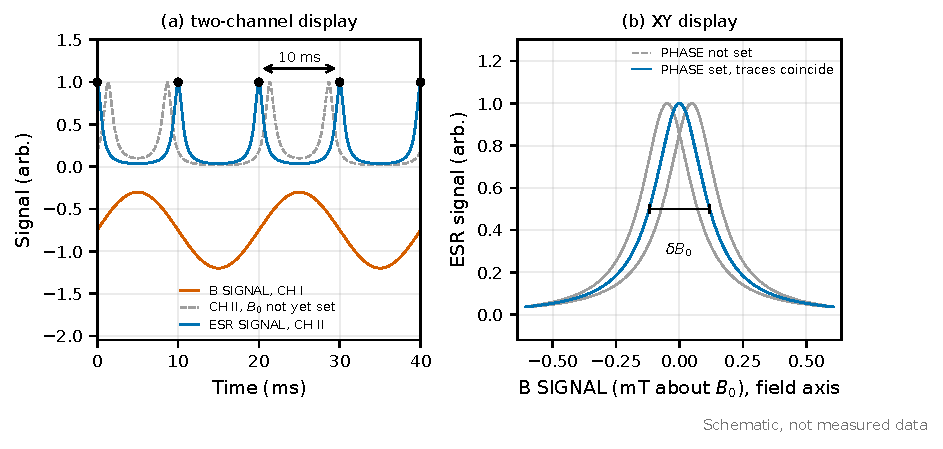
\includegraphics[width=0.82\textwidth]{figures/fig_esr_displays.pdf}
\caption{Schematic of the two ESR oscilloscope displays. Both panels are drawn from the
representative parameters of the \SI{50}{\mega\hertz} line-width measurement:
$B_0 = \SI{1.740}{\milli\tesla}$, a modulation swing of \SI{1.214}{\milli\tesla} peak to peak and
a line \SI{0.238}{\milli\tesla} wide at half height. (a) The two-channel display, with the B
SIGNAL on CH I and the ESR SIGNAL on CH II. On resonance the two absorptions per modulation cycle
are \SI{10}{\milli\second} apart, half a modulation period, and that even spacing is the null
condition used to set $I_=$; the grey trace is the same display with $B_0$ set
\SI{0.25}{\milli\tesla} low, where the signals bunch into pairs. (b) The XY display, absorption
against the field axis, with the PHASE control set so that the two traversals coincide and the
half-height width $\delta B_0$ can be read; the grey loop is the same signal with an uncompensated
lag of \SI{0.08}{\radian}. This is a schematic of the instrument display, not a captured trace and
not measured data.}
\label{fig:esrdisplays}
\end{figure}

\subsection{Calibration of the Helmholtz coils}

Following Appendix 4 of the script, the magnetometer was switched to HIGH FIELD and zeroed with
the PROBE ZERO control. The Hall probe was inserted into the standard magnet, stated as
\SI{112}{\milli\tesla} with a tolerance of \SI{1}{\percent}, and the display set to that value with
PROBE CAL. The probe was then moved to the centre of the Helmholtz pair, the instrument switched
to LOW FIELD, and the display zeroed again with the current off, which subtracts whatever ambient
field lies along the probe axis at that point, including the Earth's field. The Helmholtz current
was then set from \SI{0.1}{\ampere} to \SI{1.2}{\ampere} in \SI{0.1}{\ampere} steps and the field
read at each.

\subsection{ESR measurement procedure}

With the largest plug-in coil fitted and the DPPH sample in place, the frequency was set to
\SI{15}{\mega\hertz}, the modulation current $I_\sim$ set to mid-position and the PHASE
potentiometer turned fully to the right. The control unit display was toggled to A= and the steady
current raised slowly until the resonance signals were equally spaced. The oscilloscope was then
switched to XY mode, the phase adjusted until the two signals coincided, and the display returned
to dual mode. The steady current was trimmed for a symmetrical signal and the modulation current
reduced as far as the signal would allow.

The steady current $I_=$ and the frequency $\nu$ were recorded, the frequency increased in
\SI{5}{\mega\hertz} steps and the current readjusted at each. The measurement was repeated five
times at every frequency so that the scatter could be assessed, as the script requires. The
procedure was then repeated with the medium coil over \SIrange{35}{75}{\mega\hertz} and the
smallest coil over \SIrange{80}{130}{\mega\hertz}, giving 24 frequencies. The script warns that
sharp resonance cannot be obtained at every frequency and that some waveforms appear distorted.
In this data set a symmetric signal was obtainable at every \SI{5}{\mega\hertz} step, so no
frequency had to be discarded and all 24 points are retained. Each frequency was taken on one
plug-in coil only, so although the three bands overlap, no frequency was measured twice on two
different coils.

\subsection{Line-width procedure}
\label{sec:width}

The resonance condition was established at \SI{50}{\mega\hertz} on the medium coil and the
oscilloscope switched to XY mode with both channels at \SI{0.5}{\volt\per\centi\metre}. The
modulation current was increased until the trace spanned exactly the \SI{10.0}{\centi\metre} width
of the screen, and that root-mean-square current recorded as $I_{\mathrm{mod}}$, the corresponding
full modulation voltage being
$U_{\mathrm{mod}} = \SI{0.5}{\volt\per\centi\metre}\times\SI{10.0}{\centi\metre} = \SI{5.00}{\volt}$.
The X deflection was then expanded to \SI{0.2}{\volt\per\centi\metre} and the width $\delta U$ of
the signal at half its full height read in volts. Note that $\delta U$ is a voltage and is
therefore independent of the volts-per-centimetre setting used to read it; expanding the trace
magnifies it by a factor of $2.5$ for easier reading but does not change $\delta U$.

Since the full \SI{10}{\centi\metre} of X deflection corresponds to the peak-to-peak modulation
current, and the root-mean-square value must be multiplied by $2\sqrt{2}$ to obtain that,
the proportion carries straight across and gives the script's equation (7),
\begin{equation}
\frac{\delta I}{2\sqrt{2}\,I_{\mathrm{mod}}} = \frac{\delta U}{U_{\mathrm{mod}}}
\qquad\Longrightarrow\qquad
\delta I = 2\sqrt{2}\;I_{\mathrm{mod}}\;\frac{\delta U}{U_{\mathrm{mod}}} ,
\label{eq:eq7}
\end{equation}
after which the width in field units follows from the measured coil constant $s$ as
$\Delta B_0 = s\,\delta I$.

\subsection{NMR apparatus and procedure}

The NMR assembly comprised an NMR supply unit containing a marginal oscillator working between
about \SI{15}{\mega\hertz} and \SI{20}{\mega\hertz}, an NMR probe, a pair of electromagnet coils
with an iron yoke, separate modulation coils, a DC power supply and the oscilloscope. The
electromagnet coils were connected in series to the DC supply and the modulation coils in series
with the MODULATION COILS output. The probe was connected to the PROBE input, the DB SIGNAL output
taken to CH I of the oscilloscope and the NMR SIGNAL output to CH II, both AC coupled, with the
oscilloscope placed several inches from the magnet to avoid distortion of the display.

The HF AMPLITUDE control was set to minimum and FREQUENCY to maximum, FAST SWEEP was selected and
the modulation amplitude set to maximum. The glycerine sample tube was inserted into the measuring
chamber and its O-ring adjusted so that the sample sat at the chamber centre. The unit was
switched on and the HF amplitude raised slowly until a frequency of about \SI{19}{\mega\hertz} was
displayed, then reduced to about \SI{18.5}{\mega\hertz}. With the DC supply controls at minimum,
the coil current was brought to about \SI{3.2}{\ampere} and the frequency decreased slowly until
resonance signals appeared. The signal was optimised by varying the HF amplitude, then centred by
adjusting the coil current or the frequency while reducing the modulation amplitude. The
oscilloscope was switched to XY mode and the PHASE of the modulation voltage adjusted so that the
signals from both half-waves coincided, then returned to dual mode. The modulation frequency is
\SI{28}{\hertz}, not a harmonic or sub-harmonic of the \SI{50}{\hertz} mains supply, so that,
whatever the reason for the choice, mains pickup drifts across the trace instead of locking to it
and imitating signal. Both displays are drawn in Figure~\ref{fig:displays}.

The procedure was repeated for polystyrene, for polythene and for PTFE, and the transients
described in Section~\ref{sec:theorywiggles} recorded for each sample. Polythene and polystyrene
were then examined at a single fixed current only, because their lines were too broad and weak to
locate reliably at every set point; the full frequency-against-current run of
Section~\ref{sec:sweeprule} was taken for glycerine and for PTFE.

\subsection{Electromagnet calibration and the one-directional sweep}
\label{sec:sweeprule}

For the quantitative part, the apparatus was first tuned on glycerine, the sample removed and the
Hall probe of the teslameter inserted carefully into the measuring chamber. The field was measured
against the series coil current for an increasing sweep from \SI{3}{\ampere} to \SI{4}{\ampere}
and then for a decreasing sweep back to \SI{3}{\ampere}, in \SI{0.1}{\ampere} steps.

The two branches do not coincide, because the yoke is ferromagnetic. Magnetisation proceeds by the
motion of domain walls, which are pinned by grain boundaries, dislocations and inclusions.
Unpinning requires a finite driving field and the energy released when a wall breaks free is
dissipated, so the process is irreversible and $B$ lags behind $H$ \cite{cullity}. Sweeping the
current from \SI{3}{\ampere} to \SI{4}{\ampere} and back traces a minor loop rather than the full
major loop, because the current never reverses and never returns to zero, so the two branches
must converge at the upper turning point, and the gap is largest near the lower one.

The consequence is procedural and is stated by the script: the current must be moved in one
direction only. The calibration is single-valued on one branch only, and the subsequent frequency
run converts each current to a field using it. Backing the current off and re-approaching lands
the magnet on a different minor loop, and that error is systematic rather than random and
one-signed, so it does not average out with repetition.

The glycerine sample was returned to the chamber and the resonance frequency measured against
current from \SI{3.00}{\ampere} to \SI{4.00}{\ampere} in \SI{0.10}{\ampere} steps, the current
raised monotonically throughout. The measurement was repeated for PTFE, and finally all four
samples were compared at the single fixed current of \SI{3.50}{\ampere}.

\section{Results and analysis}

All fits in this section are least squares. The Helmholtz and electromagnet calibrations carry
uncertainty on the ordinate only, so the standard closed-form weighted expressions of
Section~\ref{sec:effvar} apply, with weights $w_i = 1/\sigma_i^{2}$. The ESR resonance fit and
both NMR frequency fits carry uncertainty on both axes, and the larger part of it sits on the
abscissa, so both use the effective-variance method of Section~\ref{sec:effvar}, iterated to
convergence, with the field uncertainty projected onto the frequency axis through the gradient.
Reduced chi-squared is quoted for every fit.

\subsection{Calibration of the Helmholtz coils}
\label{sec:helmfit}

Twelve field readings were taken from \SI{0.1}{\ampere} to \SI{1.2}{\ampere}, covering
\SIrange{0.42}{5.03}{\milli\tesla}. The full data are in Table~\ref{tab:a1}. A straight line
$B = sI + B_{\mathrm{off}}$ was fitted with $\sigma_B = \SI{0.010}{\milli\tesla}$ on every point.
The coil current is treated as exact in this fit. The same ammeter reading defines the current in
the calibration and in the resonance run, so a scale or offset error in it is common to both and
cancels in the ratio that gives the g-factor; only its random component matters, and that is
already captured in the repeat scatter of the resonance currents.
The fit is shown in Figure~\ref{fig:helm} and the results in Table~\ref{tab:helm}.

\begin{figure}[htbp]
\centering
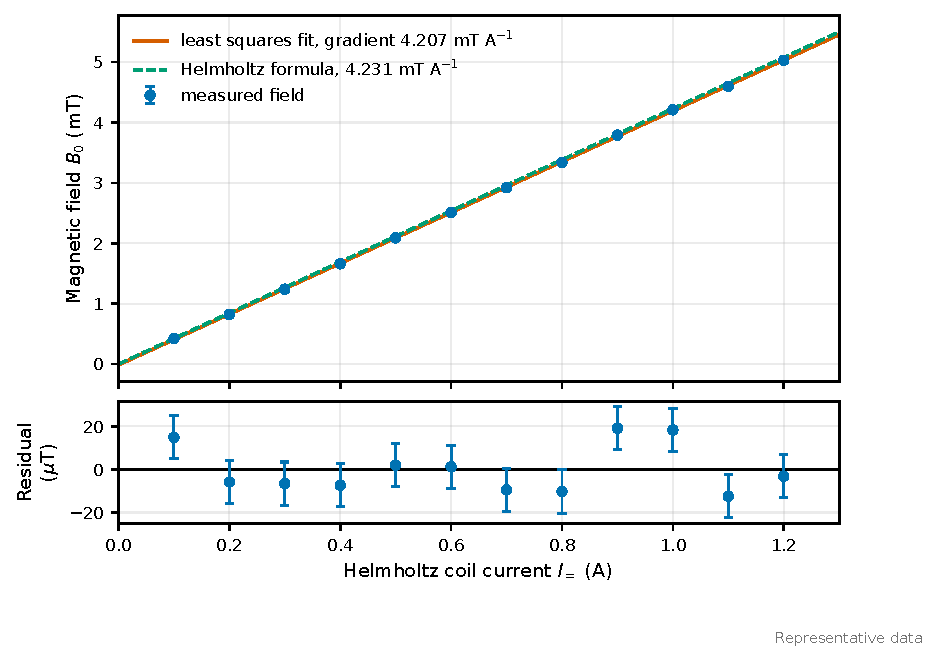
\includegraphics[width=0.60\textwidth]{figures/fig_esr_helmholtz_calibration.pdf}
\caption{Helmholtz coil calibration from representative data. Upper panel: measured field at the
coil midpoint against steady coil current, with the least squares fit and, for comparison, the
theoretical line of equation~\eqref{eq:helm}. Lower panel: fit residuals in microtesla. The
largest residual is \SI{19.0}{\micro\tesla}, about twice the assigned reading uncertainty.}
\label{fig:helm}
\end{figure}

\begin{table}[htbp]
\centering
\caption{Helmholtz calibration fit, from representative data.}
\label{tab:helm}
\footnotesize
\begin{tabular}{lll}
\toprule
Quantity & Value & Note \\
\midrule
Coil constant $s$, statistical only & \SI{4.2073 \pm 0.0084}{\milli\tesla\per\ampere} & from the fit \\
Coil constant $s$, statistical and systematic & \SI{4.207 \pm 0.043}{\milli\tesla\per\ampere} & includes \SI{1}{\percent} reference magnet \\
Intercept $B_{\mathrm{off}}$ & \SI{-0.0156 \pm 0.0062}{\milli\tesla} & residual zeroing offset \\
Chi-squared & 14.15 & 10 degrees of freedom \\
Reduced chi-squared & 1.41 & \\
Largest residual & \SI{19.0}{\micro\tesla} & \\
Theoretical value, equation~\eqref{eq:helm} & \SI{4.2314}{\milli\tesla\per\ampere} & $n = 320$, $r = \SI{6.8}{\centi\metre}$ \\
Difference from theory & \SI{-0.0241}{\milli\tesla\per\ampere}, \SI{-0.57}{\percent} & \\
Effective turns per coil implied & $318.2 \pm 3.2$ & stated value 320, consistent \\
\bottomrule
\end{tabular}
\end{table}

The fitted coil constant is \SI{0.57}{\percent} below the value predicted by the Helmholtz formula
for 320 turns. Inverting equation~\eqref{eq:helm} for the turn count gives an effective
$318.2 \pm 3.2$ turns per coil, where the uncertainty is the \SI{1.02}{\percent} on the
systematic-inclusive coil constant. The gap from 320 is therefore only 0.6 standard deviations
and the data cannot distinguish 318 from 320.
That is a plausible difference for a hand-wound coil, and it is exactly why the
script instructs that the calibration rather than the formula be used. The measured value is used
for every field in the ESR analysis. The small negative intercept is consistent with a residual
offset on the LOW FIELD zero; it shifts the field axis but not its scale.

\subsection{Resonance frequency against magnetic field, and the g-factor of DPPH}
\label{sec:esrfit}

Resonance was located at 24 frequencies from \SI{15}{\mega\hertz} to \SI{130}{\mega\hertz} across
the three plug-in coils, with five repeat settings of the current at each. The currents ran from
\SI{0.117}{\ampere} to \SI{1.099}{\ampere}, comfortably inside the range over which the coils were
calibrated, and the corresponding fields from \SI{0.477}{\milli\tesla} to
\SI{4.607}{\milli\tesla}. The mean standard error on a current was \SI{0.0024}{\ampere}. The full
data are in Table~\ref{tab:a2}. The fit is shown in Figure~\ref{fig:esrfit} and the results in
Table~\ref{tab:esrfit}.

\begin{figure}[htbp]
\centering
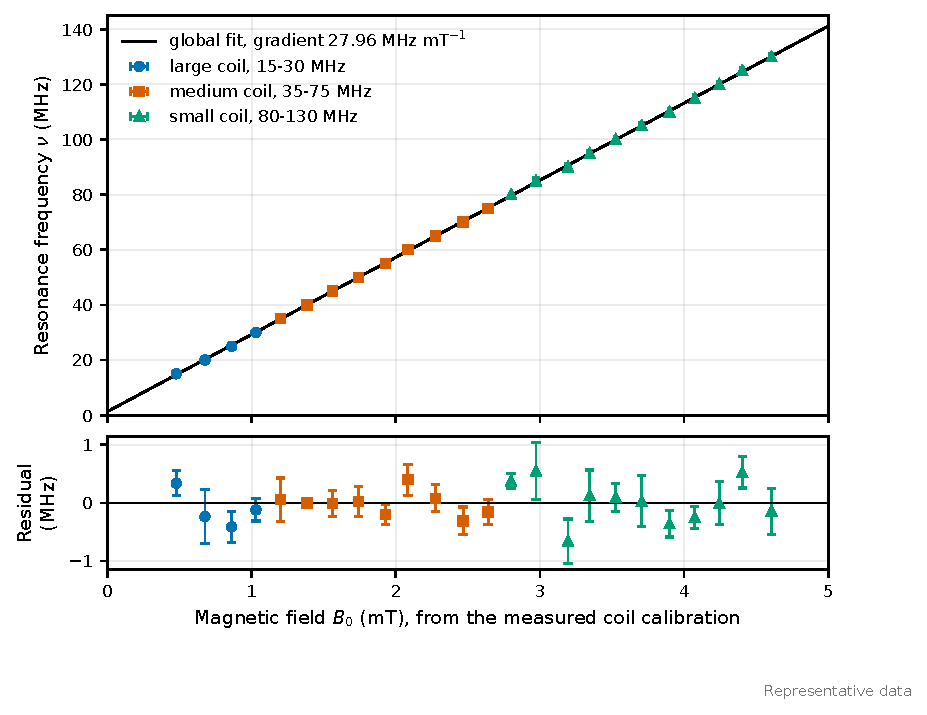
\includegraphics[width=0.62\textwidth]{figures/fig_esr_nu_vs_B.pdf}
\caption{ESR resonance frequency against magnetic field for DPPH, from representative data.
Currents have been converted to field with the measured coil constant of
Table~\ref{tab:helm}. The three plug-in coils are distinguished by symbol. The line is a single
global weighted fit to all 24 points. The lower panel shows the residuals, which scatter about
zero and show no offset between the three coil bands beyond what the point scatter allows,
although no frequency was measured on two coils, so a common offset smaller than about
\SI{0.1}{\mega\hertz} would not have been detected.}
\label{fig:esrfit}
\end{figure}

\begin{table}[htbp]
\centering
\caption{ESR resonance fit and the extracted g-factor of DPPH, from representative data.}
\label{tab:esrfit}
\footnotesize
\begin{tabular}{@{}L{4.8cm}L{7.4cm}L{3.5cm}@{}}
\toprule
Quantity & Value & Note \\
\midrule
Gradient $\mathrm{d}\nu/\mathrm{d}B_0$ & \SI{27.963 \pm 0.045}{\mega\hertz\per\milli\tesla} & fit only, calibration uncertainty not included \\
\textbf{Gradient, quoted result} & \SI{27.963 \pm 0.071}{\mega\hertz\per\milli\tesla} & statistical, calibration included \\
Intercept $\nu_0$ & \SI{1.333 \pm 0.114}{\mega\hertz} & \\
Chi-squared, reduced chi-squared & 26.18, 1.19 & 22 degrees of freedom \\
Largest residual & \SI{0.662}{\mega\hertz} & \\
Gradient $\mathrm{d}\nu/\mathrm{d}I_=$ & \SI{117.65 \pm 0.19}{\mega\hertz\per\ampere} & consistency check on the error propagation \\
$k/s$ from the two gradients & \SI{27.96 \pm 0.07}{\mega\hertz\per\milli\tesla} & agrees identically, as it must \\
\midrule
$g_s$(DPPH), central value & 1.9979 & equation~\eqref{eq:gwork} \\
Statistical uncertainty & 0.0051 & fit and calibration combined \\
Systematic uncertainty & 0.0200 & \SI{1}{\percent} reference magnet \\
\textbf{Quoted result} & $\mathbf{1.998 \pm 0.005\,(\text{stat}) \pm 0.020\,(\text{syst})}$ \newline $\mathbf{= 1.998 \pm 0.021}$ & \SI{1.03}{\percent} \\
\midrule
Literature $g$(DPPH), and difference & $2.0036 \pm 0.0002$; \SI{-0.29}{\percent}, $0.28\sigma$ & \cite{krzystek} \\
Free electron $g_e$, and difference & 2.002319304; \SI{-0.22}{\percent}, $0.22\sigma$ & \cite{codata} \\
\bottomrule
\end{tabular}
\end{table}

The plot is linear over an eightfold range of frequency and a nearly tenfold range of field.
Both the field and the frequency carry uncertainty, the field through the repeat scatter of the
resonance current and the frequency through the \SI{0.1}{\mega\hertz} readout resolution and
short-term drift of the oscillator, so the effective-variance method is used. The frequency term
is not negligible: it is comparable to the projected field error at the low-field end, and
omitting it would understate the gradient uncertainty by about a fifth and inflate the reduced
chi-squared from 1.19 to 1.50. Applying equation~\eqref{eq:gwork} with
$h/\mu_B = \SI{7.144774e-11}{\tesla\second}$ gives $g_s = 1.9979$. Combining the statistical
uncertainty of $0.0051$ with the \SI{1}{\percent} systematic from the reference magnet gives a
total of $0.0206$, so the result is quoted as
\begin{equation}
g_s(\mathrm{DPPH}) = 1.998 \pm 0.005\,(\mathrm{stat}) \pm 0.020\,(\mathrm{syst}) = 1.998 \pm 0.021 .
\end{equation}
A useful cross-check is to fit $\nu$ against current directly and divide by the coil constant.
That gives \SI{117.65 \pm 0.19}{\mega\hertz\per\ampere} and hence the same
\SI{27.963}{\mega\hertz\per\milli\tesla}, as it must algebraically, but with a larger
uncertainty of \SI{0.071}{\mega\hertz\per\milli\tesla} because the calibration error is then
carried explicitly, whereas the direct fit of $\nu$ against $B_0$ uses field uncertainties built
only from the current scatter and so omits it entirely. The two routes are not independent
determinations; the second is the one that carries the full statistical error and it is the one
propagated into $g$. The direct fit supplies the central value, and the two-gradient route
supplies the uncertainty, so the $0.0051$ statistical uncertainty on $g_s$ comes from the latter.

The fitted intercept deserves attention because the physics requires it to be zero: an $S = 1/2$
system has no zero-field splitting, since the term responsible vanishes identically for a
doublet. The measured intercept of \SI{1.333 \pm 0.114}{\mega\hertz} is 12 standard deviations
from zero, so it is not consistent with zero. Dividing by the gradient converts it into a field.
Relative to the calibrated axis the excess at the DPPH sample is
\SI{+0.048 \pm 0.004}{\milli\tesla}; once the calibration's own zero offset of
\SI{-0.016}{\milli\tesla} is removed, the implied ambient field along the coil axis is
\SI{+0.032}{\milli\tesla}. That is the right size for the residual ambient field left
after zeroing the magnetometer at the coil centre. Only the axial component matters, and in
Glasgow the Earth's field of about \SI{48}{\micro\tesla} is steeply inclined, so a horizontal
coil axis sees roughly \SI{17}{\micro\tesla} of it; the balance is stray field from nearby
equipment. An offset of this kind shifts the intercept and leaves the
gradient untouched, which is precisely why the g-factor is taken from the gradient. The intercept
is therefore reported as a diagnostic rather than forced to zero.

\subsection{Line width of the DPPH resonance}
\label{sec:widthres}

The width was measured at \SI{50}{\mega\hertz} on the medium plug-in coil, where the resonance
current was \SI{0.417}{\ampere} and the field \SI{1.7397 \pm 0.0092}{\milli\tesla}. The measured
quantities and the values derived from equation~\eqref{eq:eq7} are in Table~\ref{tab:width}, and
the line shape with the half-height construction drawn on it is in Figure~\ref{fig:width}.

\begin{figure}[htbp]
\centering
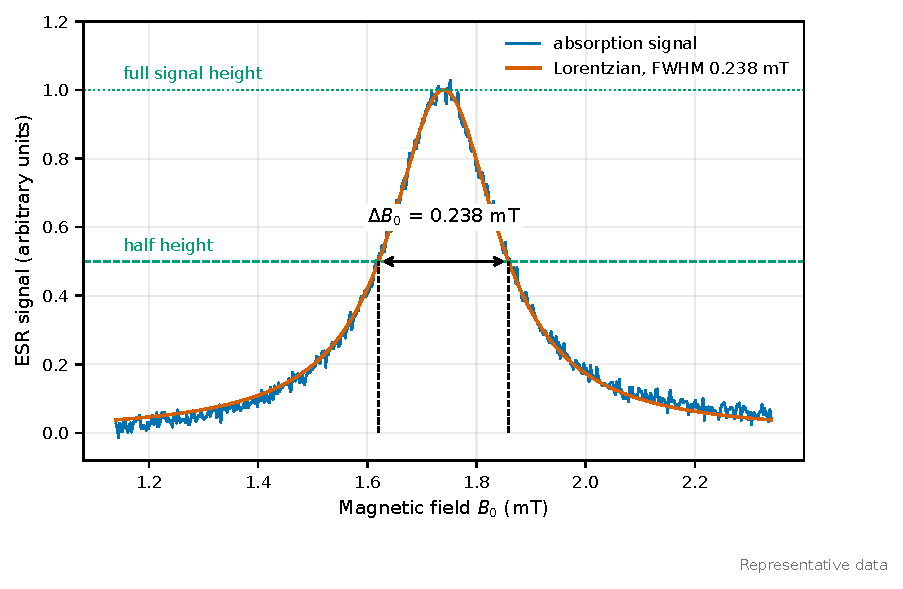
\includegraphics[width=0.56\textwidth]{figures/fig_esr_linewidth.pdf}
\caption{DPPH absorption line at \SI{50}{\mega\hertz} with the half-height width construction,
from representative data. The horizontal axis is the field axis provided by the oscilloscope XY
display once the PHASE control has been set for coincidence of the two half-wave traces. The
smooth curve is a Lorentzian of full width \SI{0.238}{\milli\tesla} at half maximum.}
\label{fig:width}
\end{figure}

\begin{table}[htbp]
\centering
\caption{Line-width measurement at \SI{50}{\mega\hertz}, from representative data.}
\label{tab:width}
\footnotesize
\begin{tabular}{llll}
\toprule
Quantity & Value & Uncertainty & Note \\
\midrule
RF frequency & \SI{50.0}{\mega\hertz} & \SI{0.1}{\mega\hertz} & set value, medium coil \\
Resonance current $I_=$ & \SI{0.417}{\ampere} & \SI{0.0022}{\ampere} & mean of five repeats \\
Resonance field $B_0$ & \SI{1.7397}{\milli\tesla} & \SI{0.0092}{\milli\tesla} & from the calibration \\
Modulation current $I_{\mathrm{mod}}$ (RMS) & \SI{0.102}{\ampere} & \SI{0.005}{\ampere} & trace spans \SI{10.0}{\centi\metre} \\
Full modulation voltage $U_{\mathrm{mod}}$ & \SI{5.00}{\volt} & \SI{0.10}{\volt} & \SI{0.5}{\volt\per\centi\metre} over \SI{10.0}{\centi\metre} \\
Half-height width $\delta U$ & \SI{0.98}{\volt} & \SI{0.05}{\volt} & read at \SI{0.2}{\volt\per\centi\metre} \\
Half-width current $\delta I$ & \SI{0.0565}{\ampere} & \SI{0.0042}{\ampere} & equation~\eqref{eq:eq7} \\
\textbf{Line width $\Delta B_0$ (FWHM)} & \textbf{\SI{0.238}{\milli\tesla}} & \textbf{\SI{0.018}{\milli\tesla}} & \SI{7.4}{\percent} \\
Same, in gauss & \SI{2.38}{\gauss} & \SI{0.18}{\gauss} & \\
Peak-to-peak derivative width & \SI{0.137}{\milli\tesla} & \SI{0.010}{\milli\tesla} & equation~\eqref{eq:pp} \\
Same, in gauss & \SI{1.37}{\gauss} & \SI{0.10}{\gauss} & for literature comparison \\
Relaxation time $T_2$ & \SI{47.8}{\nano\second} & \SI{3.6}{\nano\second} & equation~\eqref{eq:t2} \\
\bottomrule
\end{tabular}
\end{table}

Three internal consistency checks were made on this measurement, all of which the data pass. The
peak-to-peak modulation field, $s \times 2\sqrt{2} \times I_{\mathrm{mod}} =
\SI{1.214}{\milli\tesla}$, stays below the steady field of \SI{1.7397}{\milli\tesla}, so the field
never reverses and the two-crossings-per-cycle picture holds. The line occupies
\SI{20}{\percent} of the \SI{10}{\centi\metre} trace, that is \SI{2.0}{\centi\metre} at
\SI{0.5}{\volt\per\centi\metre}, expanding to \SI{4.9}{\centi\metre} at
\SI{0.2}{\volt\per\centi\metre}. Both are comfortably readable on a real screen.

Because $\Delta B_0 = s\,\delta I$, the \SI{1}{\percent} field-standard systematic scales the line
width as well as the g-factors, and it is already carried inside the \SI{7.4}{\percent} quoted
above. It contributes only \SI{1.0}{\percent} of that total, against \SI{5.1}{\percent} from
$\delta U$ and \SI{4.9}{\percent} from $I_{\mathrm{mod}}$, so the width is limited by reading the
trace rather than by the field standard.

Applying equation~\eqref{eq:t2} with the fitted $g$ gives $T_2 = \SI{47.8 \pm 3.6}{\nano\second}$,
or a relaxation rate of $1/T_2 = \SI{2.090e7}{\per\second}$. This conversion assumes the line is
homogeneously broadened and Lorentzian. Any residual inhomogeneous broadening means the measured
width gives $T_2^{*}$ rather than $T_2$, so the quoted figure is properly a lower bound on the
true transverse relaxation time.

\subsection{Calibration of the electromagnet and its hysteresis}
\label{sec:magfit}

Eleven points were taken on each branch from \SI{3.00}{\ampere} to \SI{4.00}{\ampere}. The full
data are in Table~\ref{tab:a3}. The rising branch was fitted with a quadratic
$B(I) = a_0 + a_1 I + a_2 I^{2}$ by effective-variance weighted least squares, the current
uncertainty being projected onto the field axis through $\mathrm{d}B/\mathrm{d}I$. Results are in
Table~\ref{tab:mag} and the fit in Figure~\ref{fig:mag}.

\begin{figure}[htbp]
\centering
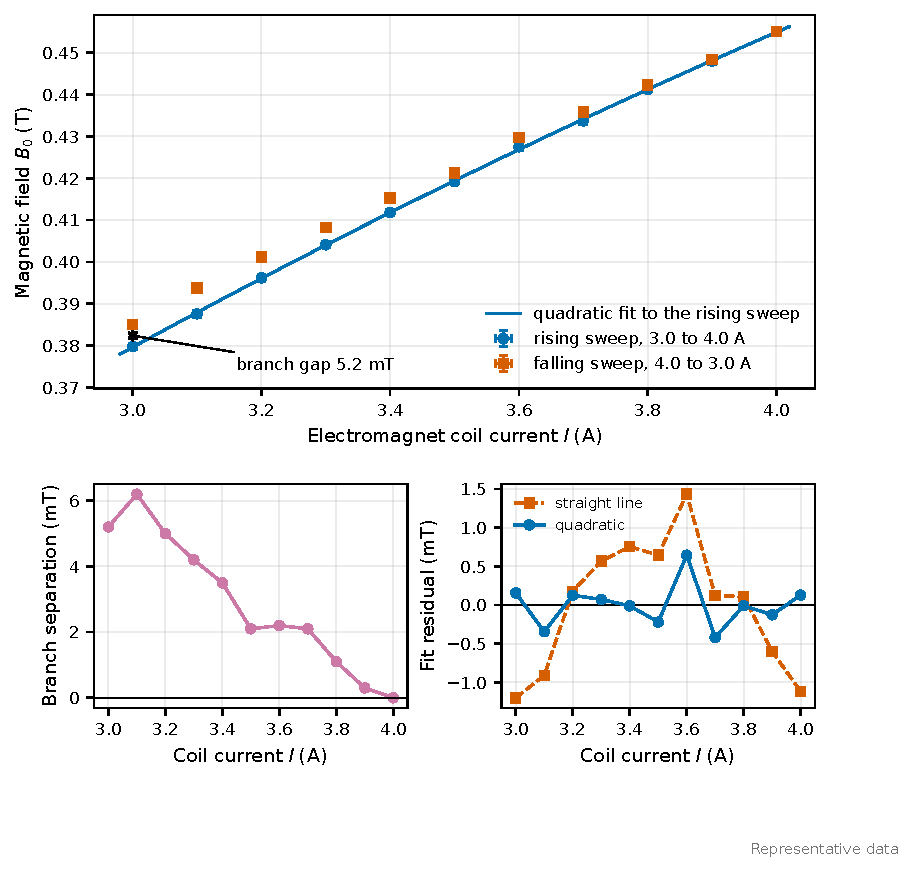
\includegraphics[width=0.58\textwidth]{figures/fig_nmr_magnet_calibration.pdf}
\caption{Electromagnet calibration from representative data. Upper panel: both sweep branches with
the quadratic fitted to the rising branch, and the branch gap at \SI{3.00}{\ampere} marked. Lower
left: the separation between the two branches, which is largest near the lower end of the sweep
and closes at the upper turning point. Lower right: residuals to a straight line and to the
quadratic. The
straight-line residuals show the systematic curvature that justifies the higher order.}
\label{fig:mag}
\end{figure}

\begin{table}[htbp]
\centering
\caption{Electromagnet calibration on the rising branch, and the model comparison, from
representative data.}
\label{tab:mag}
\footnotesize
\begin{tabular}{@{}L{4.8cm}L{7.0cm}L{3.9cm}@{}}
\toprule
Quantity & Value & Note \\
\midrule
$a_0$ & \SI{0.050 \pm 0.026}{\tesla} & not a remanent field, see text \\
$a_1$ & \SI{0.136 \pm 0.015}{\tesla\per\ampere} & \\
$a_2$ & \SI{-0.0087 \pm 0.0021}{\tesla\per\ampere\squared} & $4.0\sigma$ from zero \\
Chi-squared, quadratic & 2.15 & 8 degrees of freedom \\
Reduced chi-squared, quadratic & 0.27 & \\
Largest quadratic residual & \SI{0.64}{\milli\tesla} & \\
Reduced chi-squared, straight line & 2.06 & 9 degrees of freedom \\
Largest straight-line residual & \SI{1.43}{\milli\tesla} & against \SI{0.5}{\milli\tesla} scatter \\
Improvement in chi-squared on adding $I^{2}$ & 16.4 & one extra parameter, $F = 61.0$ \\
Cubic coefficient $a_3$ & \SI{0.0008 \pm 0.0080}{\tesla\per\ampere\cubed} & $0.10\sigma$, consistent with zero \\
Improvement in chi-squared on adding $I^{3}$ & 0.01 & $F = 0.03$, not justified \\
\midrule
$\mathrm{d}B/\mathrm{d}I$ at 3.00, 3.50, \SI{4.00}{\ampere} & \SI{0.0839 \pm 0.0022}{}, \SI{0.0752 \pm 0.0006}{}, \SI{0.0666 \pm 0.0022}{\tesla\per\ampere} & falls by \SI{20.6}{\percent}, yoke saturation \\
Field at 3.00, 3.50, \SI{4.00}{\ampere} & \SI{0.3796}{\tesla}, \SI{0.4194}{\tesla}, \SI{0.4549}{\tesla} & \\
\midrule
Branch separation at 3.00, 3.50, \SI{4.00}{\ampere} & \SI{5.2}{\milli\tesla}, \SI{2.1}{\milli\tesla}, \SI{0.0}{\milli\tesla} & \SI{1.37}{\percent} of $B$ at \SI{3.00}{\ampere}; branches meet at the top \\
Equivalent proton frequency shift at \SI{3.00}{\ampere} & \SI{0.221}{\mega\hertz} & 11 times the setting precision \\
\bottomrule
\end{tabular}
\end{table}

Three points follow. First, the order of the polynomial is justified rather than assumed. The
magnetic circuit argument requires $\mathrm{d}B/\mathrm{d}I$ to fall with current, so any adequate
model must have negative curvature, and a quadratic is the lowest order that can provide it. A
straight line leaves residuals with obvious systematic curvature, largest at
\SI{1.43}{\milli\tesla} against a point scatter of \SI{0.5}{\milli\tesla}, and a reduced
chi-squared of 2.06. Adding the quadratic term improves chi-squared by 16.4 for one extra
parameter, an $F$ statistic of 61.0, while adding a cubic improves it by 0.01, an $F$ statistic of
0.03, with the cubic coefficient itself $0.10\sigma$ from zero. The quadratic is the right model
and the cubic is not justified.

Second, the reduced chi-squared of 0.27 means the assigned uncertainties are slightly conservative
rather than that the fit is suspect: the teslameter scatter of \SI{0.5}{\milli\tesla} and the
current reading uncertainty of \SI{0.005}{\ampere} were both assessed before the run rather than
inferred from the residuals.

Third, the fitted intercept $a_0 = \SI{0.0501}{\tesla}$ is \emph{not} a remanent field but an
extrapolation from \SI{3}{\ampere} back to \SI{0}{\ampere}, far outside the range fitted. Real
remanence for a magnet of this kind would be \SIrange{10}{30}{\milli\tesla}, several times
smaller. The quadratic is a local empirical interpolation, in effect a Taylor expansion of the true
$B(I)$ truncated at second order, and must not be used outside \SIrange{3.0}{4.0}{\ampere}.

The hysteresis is large enough to matter. The branch separation of \SI{5.2}{\milli\tesla} at
\SI{3.00}{\ampere} is \SI{1.37}{\percent} of the field there and corresponds to a proton
resonance shift of \SI{0.221}{\mega\hertz}, eleven times the precision with which the frequency
can be set, and it closes to zero at the upper turning point as a minor loop must. The largest
separation observed was \SI{6.2}{\milli\tesla} at \SI{3.10}{\ampere}, the \SI{5.2}{\milli\tesla}
quoted at \SI{3.00}{\ampere} being one reading of the same quantity, limited by the
\SI{0.5}{\milli\tesla} reading scatter. This is the
quantitative justification for the one-directional sweep rule of Section~\ref{sec:sweeprule}.

\subsection{The g-factors of the proton and of fluorine}
\label{sec:nmrfit}

Resonance frequencies were recorded against current for glycerine and for PTFE on the rising
branch only, eleven points each. Glycerine gave \SIrange{16.14}{19.37}{\mega\hertz} and PTFE
\SIrange{15.28}{18.31}{\mega\hertz}, both inside the oscillator's stated band. Each current was
converted to a field with the quadratic of Section~\ref{sec:magfit}, carrying the full propagated
uncertainty including all three coefficient covariances and the current setting error, which gives
a mean field uncertainty of \SI{0.50}{\milli\tesla}. The frequency scatter was taken as
\SI{0.020}{\mega\hertz} for glycerine and \SI{0.050}{\mega\hertz} for PTFE, set by the display
resolution and the short-term drift of the marginal oscillator. The full data are in
Table~\ref{tab:a4}. The fits are in Figure~\ref{fig:nmrfit} and the results in
Table~\ref{tab:nmrfit}.

\begin{figure}[htbp]
\centering
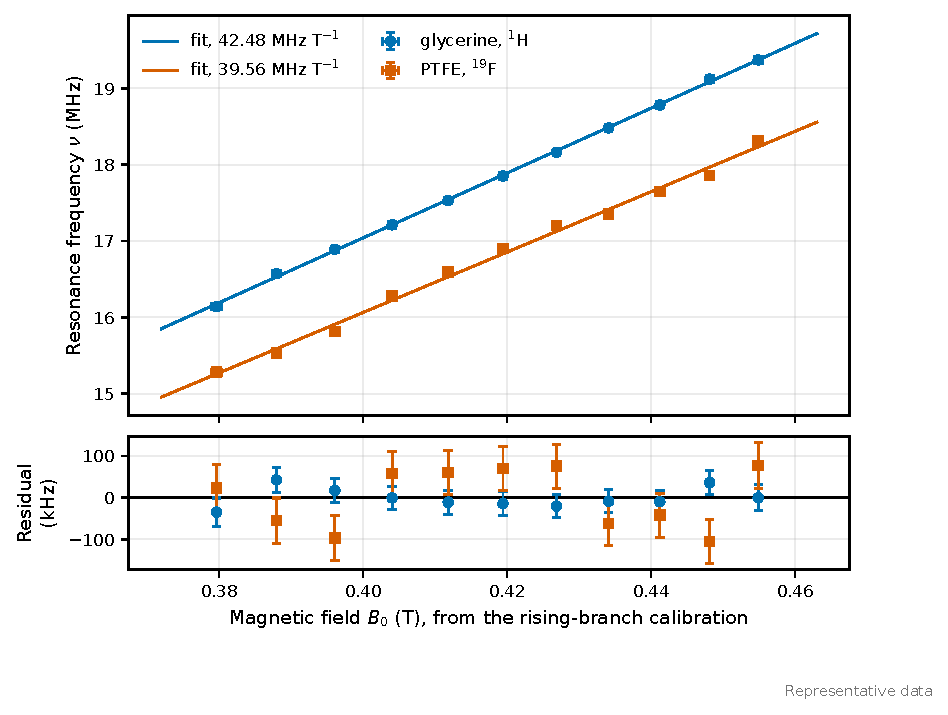
\includegraphics[width=0.62\textwidth]{figures/fig_nmr_nu_vs_B.pdf}
\caption{NMR resonance frequency against magnetic field for protons in glycerine and fluorine in
PTFE, from representative data. Fields come from the rising-branch quadratic calibration of
Figure~\ref{fig:mag}. Lower panel: fit residuals in kilohertz. The PTFE residuals are visibly
larger than the glycerine residuals, as the difference in the assumed frequency scatter
requires.}
\label{fig:nmrfit}
\end{figure}

\begin{table}[htbp]
\centering
\caption{NMR gradients and g-factors for $^{1}$H in glycerine and $^{19}$F in PTFE, from
representative data.}
\label{tab:nmrfit}
\footnotesize
\begin{tabular}{@{}L{5.0cm}L{5.3cm}L{5.3cm}@{}}
\toprule
Quantity & $^{1}$H in glycerine & $^{19}$F in PTFE \\
\midrule
Frequency range & \SIrange{16.14}{19.37}{\mega\hertz} & \SIrange{15.28}{18.31}{\mega\hertz} \\
Assumed frequency scatter & \SI{0.020}{\mega\hertz} & \SI{0.050}{\mega\hertz} \\
Mean propagated field uncertainty & \SI{0.50}{\milli\tesla} & \SI{0.50}{\milli\tesla} \\
Gradient $\mathrm{d}\nu/\mathrm{d}B_0$, route A & \SI{42.48 \pm 0.38}{\mega\hertz\per\tesla} & \SI{39.56 \pm 0.69}{\mega\hertz\per\tesla} \\
Relative statistical uncertainty & \SI{0.90}{\percent} & \SI{1.74}{\percent} \\
Intercept $c$, and its significance & \SI{0.05 \pm 0.16}{\mega\hertz}, $0.30\sigma$ & \SI{0.24 \pm 0.29}{\mega\hertz}, $0.83\sigma$ \\
Implied extra field $c/m$ & \SI{+1.1 \pm 3.8}{\milli\tesla} & \SI{+6.1 \pm 7.3}{\milli\tesla} \\
Chi-squared, reduced chi-squared (9 dof) & 6.22, 0.69 & 18.62, 2.07 \\
Largest residual & \SI{43}{\kilo\hertz} & \SI{106}{\kilo\hertz} \\
Gradient, route B at \SI{3.50}{\ampere} & \SI{42.53 \pm 0.42}{\mega\hertz\per\tesla} & \SI{39.57 \pm 0.71}{\mega\hertz\per\tesla} \\
$\mathrm{d}\nu/\mathrm{d}I$ at \SI{3.50}{\ampere} & \SI{3.199 \pm 0.019}{\mega\hertz\per\ampere} & \SI{2.976 \pm 0.048}{\mega\hertz\per\ampere} \\
Gradient, Monte Carlo cross-check & \SI{42.51 \pm 0.42}{\mega\hertz\per\tesla} & \SI{39.58 \pm 0.70}{\mega\hertz\per\tesla} \\
Literature gradient, and difference & \SI{42.5775}{\mega\hertz\per\tesla}, \SI{-0.23}{\percent} & \SI{40.0776}{\mega\hertz\per\tesla}, \SI{-1.30}{\percent} \\
\midrule
$g$, central value & 5.5726 & 5.1892 \\
Statistical uncertainty & 0.0503 & 0.0904 \\
Systematic uncertainty & 0.0557 & 0.0519 \\
\textbf{Quoted result} & $\mathbf{5.57 \pm 0.08}$ & $\mathbf{5.19 \pm 0.10}$ \\
Total relative uncertainty & \SI{1.35}{\percent} & \SI{2.01}{\percent} \\
Literature $g$ & 5.585695 & 5.257736 \\
Difference & \SI{-0.23}{\percent}, $0.17\sigma$ & \SI{-1.30}{\percent}, $0.66\sigma$ \\
\bottomrule
\end{tabular}
\end{table}

Applying equation~\eqref{eq:nmrres} gives $g(^{1}\mathrm{H}) = 5.57 \pm 0.08$ and
$g(^{19}\mathrm{F}) = 5.19 \pm 0.10$. Both agree with the literature values of 5.5857
\cite{codata} and 5.2577 \cite{stone,harris}, at $0.17\sigma$ and $0.66\sigma$ respectively.

Three ways of propagating the same data and the same calibration were compared, and they agree;
they test the error propagation rather than provide independent determinations. The one
independent test is the gradient ratio below, in which the field scale cancels. Route A, quoted as
the result, fits $\nu$ against $B_0$ over the whole field span using the effective-variance method.
Route B, which follows the chain rule the script's wording suggests, fits $\nu$ against current
directly and divides the two local gradients at \SI{3.50}{\ampere}. Route B is systematically the
more conservative of the two, because it evaluates a local gradient at one current and discards
the lever arm of the full range: for the proton it gives \SI{0.99}{\percent} against
\SI{0.90}{\percent}. A Monte Carlo sampling of the calibration covariance over 5000 draws returned
\SI{42.51 \pm 0.42}{\mega\hertz\per\tesla} for the proton, in agreement with both.

A further test cancels the correlated field scale entirely. The ratio of the two fitted gradients
is $0.9312 \pm 0.0183$, against the literature ratio $40.0776/42.5775 = 0.94129$, a difference of
\SI{1.07}{\percent} and $0.55\sigma$. Because both gradients were measured against the same
calibrated field, the \SI{1}{\percent} reference magnet uncertainty divides out of the ratio, so
this is a genuinely independent check of the two nuclear moments against each other.

Both intercepts are consistent with zero, at $0.30\sigma$ and $0.83\sigma$. Converting them into
field offsets gives \SI{+1.1 \pm 3.8}{\milli\tesla} and \SI{+6.1 \pm 7.3}{\milli\tesla},
neither significant. No probe-zero error or remanence offset was therefore detected at the level
the data can resolve, which is a few milliteslas.

\subsection{Comparison of the four samples and identification of polythene}
\label{sec:samples}

All four samples were compared at the fixed current of \SI{3.50}{\ampere}, corresponding to
\SI{0.4194 \pm 0.0005}{\tesla}. At that field the two candidate nuclei are predicted to resonate
at \SI{17.858}{\mega\hertz} for $^{1}$H and \SI{16.809}{\mega\hertz} for $^{19}$F, a separation of
\SI{1.049}{\mega\hertz} or \SI{5.87}{\percent}. Results are in Table~\ref{tab:samples} and
Figure~\ref{fig:samples}.

\begin{table}[htbp]
\centering
\caption{Four-sample comparison at \SI{3.50}{\ampere} and \SI{0.4194}{\tesla}, from representative
data. The glycerine and PTFE frequencies here are independent settings from those at
\SI{3.50}{\ampere} in Table~\ref{tab:a4}; the differences of \SI{0.02}{\mega\hertz} are one
standard deviation of the frequency-setting scatter. The last column gives the overall line width
and the number of transients counted; the widths are compared with the transient counts through
equation~\eqref{eq:wiggles} in the text.}
\label{tab:samples}
\footnotesize
\begin{tabular}{lllll}
\toprule
Sample & Formula & Nucleus & Observed $\nu$ (\si{\mega\hertz}) & Line width (\si{\milli\tesla}), wiggles \\
\midrule
glycerine & C$_3$H$_5$(OH)$_3$ & $^{1}$H & $17.87 \pm 0.02$ & 0.010, 4 to 6 and strong \\
polystyrene & (C$_8$H$_8$)$_n$ & $^{1}$H & $17.81 \pm 0.12$ & 0.500, none \\
polythene & (C$_2$H$_4$)$_n$ & $^{1}$H (deduced) & $17.80 \pm 0.05$ & 0.150 composite, 1 to 2 and weak \\
PTFE & (C$_2$F$_4$)$_n$ & $^{19}$F & $16.88 \pm 0.05$ & 0.150, none \\
\midrule
\multicolumn{3}{l}{Prediction for $^{1}$H at this field} & 17.858 & \\
\multicolumn{3}{l}{Prediction for $^{19}$F at this field} & 16.809 & \\
\multicolumn{3}{l}{Separation of the two hypotheses} & 1.049 & \SI{5.87}{\percent} \\
\bottomrule
\end{tabular}
\end{table}

\begin{figure}[htbp]
\centering
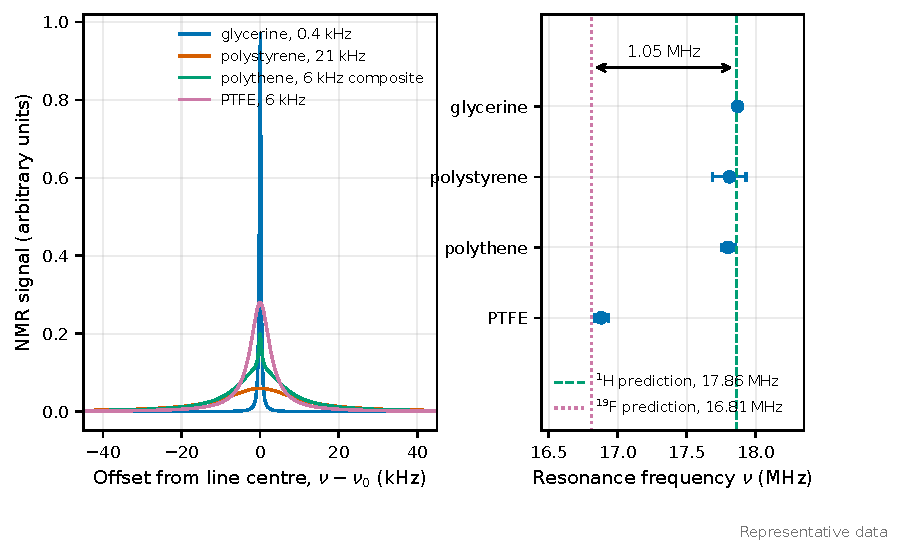
\includegraphics[width=0.70\textwidth]{figures/fig_nmr_sample_comparison.pdf}
\caption{Four-sample comparison at \SI{3.50}{\ampere}, from representative data. Left: line shapes
on a common frequency offset axis, showing the very narrow glycerine line, the broad polystyrene
line, and the intermediate PTFE and composite polythene lines. Right: observed resonance
frequencies against the two predictions. Glycerine, polystyrene and polythene fall on the proton
line and only PTFE falls on the fluorine line.}
\label{fig:samples}
\end{figure}

The polythene line was observed at \SI{17.80 \pm 0.05}{\mega\hertz}. It lies
\SI{0.058}{\mega\hertz}
from the proton prediction and \SI{0.991}{\mega\hertz} from the fluorine prediction. Both
predictions are proportional to the calibrated field, which carries the \SI{1}{\percent}
reference-magnet scale error, that is \SI{0.179}{\mega\hertz} on the proton prediction and
\SI{0.168}{\mega\hertz} on the fluorine one, so the honest significances are about 0.3 standard
deviations from the proton prediction and about 5 standard deviations from the fluorine one. Both
are dominated by that field uncertainty, which shifts the two predictions together. The
comparison that removes it is with the observed lines: polythene sits \SI{0.070}{\mega\hertz}
from the glycerine line and \SI{0.920}{\mega\hertz} from the PTFE line. Polythene therefore
contains hydrogen and contains no fluorine. The handbook formula, (C$_2$H$_4$)$_n$
\cite{crc}, confirms the deduction.

Polystyrene was observed at \SI{17.81 \pm 0.12}{\mega\hertz}, which is \SI{0.048}{\mega\hertz}
from the proton prediction, that is 0.4 standard deviations of its own measurement uncertainty.
The larger uncertainty reflects the difficulty of centring so broad and weak a line.

Two further observations support it. No second line was found anywhere in the oscillator's range:
if polythene contained both nuclei, two resonances separated by more than a megahertz would have
appeared. And carbon is silent, because $^{12}$C has even proton and neutron numbers and therefore
zero spin. The only other candidate, $^{13}$C, is spin one-half but is present at about
\SI{1}{\percent} abundance and resonates far below the oscillator's band at this field, so it
cannot be confused with anything.

Polythene and PTFE are exact structural analogues, the same backbone with every hydrogen replaced
by fluorine, which is what makes them such a clean pair for this comparison. The line shape gives a
secondary clue that is consistent with the identification. The polythene line is clearly broader
than glycerine's but noticeably narrower than polystyrene's and has a composite appearance, a
narrow component on a broad base. Polythene is semicrystalline with a glass transition far below
room temperature, so its amorphous fraction is mobile enough to narrow the dipolar coupling while
the crystalline lamellae stay rigid. Polystyrene is a glass well below its transition and is
uniformly rigid, which is why it shows only the broad component and no wiggles at all.

The two oscilloscope displays and the transient train are drawn in Figure~\ref{fig:displays}, and
the wiggle counts in Table~\ref{tab:samples} follow equation~\eqref{eq:wiggles} quantitatively.
With $\mathrm{d}B/\mathrm{d}t = \SI{0.42}{\tesla\per\second}$, glycerine's
\SI{0.010}{\milli\tesla} line gives $T_2^{*} = \SI{748}{\micro\second}$ and $N = 5.0$, which is
the four to six observed. Polythene's transients are controlled not by its overall
\SI{0.150}{\milli\tesla} width but by the narrow amorphous component of about
\SI{0.020}{\milli\tesla}, giving $T_2^{*} = \SI{374}{\micro\second}$ and $N = 1.3$, the one or two
weak ones observed. PTFE at \SI{0.150}{\milli\tesla} gives $N = 0.02$ and polystyrene at
\SI{0.500}{\milli\tesla} gives $N = 0.002$, so neither can show even one, which is what was seen.

\begin{figure}[htbp]
\centering
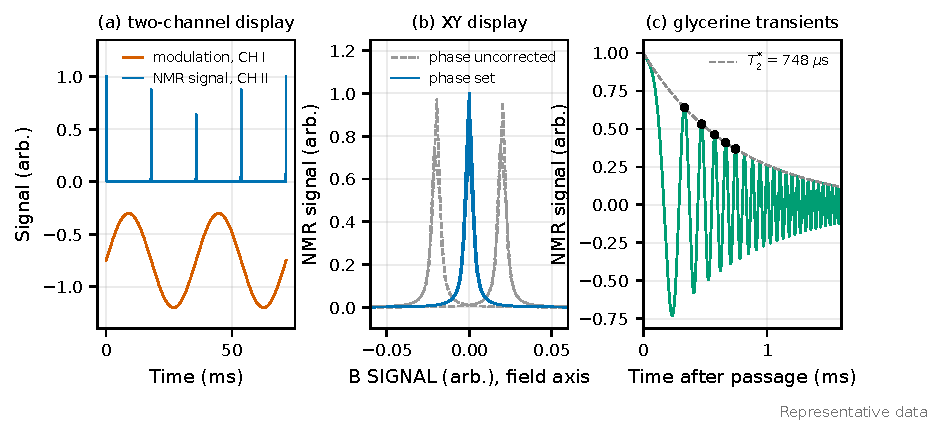
\includegraphics[width=0.94\textwidth]{figures/fig_nmr_displays_wiggles.pdf}
\caption{The NMR displays and the transients, from representative data. (a) The two-channel
display: the NMR absorption on CH II and the modulation reference on CH I, with two absorptions
per modulation cycle, evenly spaced when $B_0$ is on resonance. (b) The same signal in XY mode
with the PHASE control set so that the two half-wave traces coincide, which is the condition
under which the X axis is a faithful field axis. (c) The glycerine transient train after passage
through resonance, with the successive maxima of
$t_n = \sqrt{4\pi n/\gamma|\mathrm{d}B/\mathrm{d}t|}$ marked, showing the predicted crowding as
the envelope decays with $T_2^{*}$.}
\label{fig:displays}
\end{figure}

\section{Uncertainties}
\label{sec:unc}

\subsection{Random uncertainties}

Random uncertainties were assessed from the repeat readings where repeats were taken, and from
instrument resolution otherwise. Table~\ref{tab:random} lists them.

\begin{table}[htbp]
\centering
\caption{Random uncertainty contributions, from representative data.}
\label{tab:random}
\footnotesize
\begin{tabular}{@{}L{3.2cm}L{2.6cm}L{9.8cm}@{}}
\toprule
Quantity & Size & Origin \\
\midrule
$I_=$ at ESR resonance & \SI{0.0024}{\ampere} mean standard error & standard error of five repeats; limited by how finely the eye can judge equal spacing against a line width of \SI{0.238}{\milli\tesla}, that is \SI{0.057}{\ampere} \\
ESR frequency $\nu$ & \SI{0.1}{\mega\hertz} & readout resolution and short-term oscillator drift; carried in the fit weights \\
ESR field in the calibration & \SI{0.010}{\milli\tesla} & magnetometer display resolution and noise \\
ESR calibration current $I_=$ & treated as exact & the same ammeter serves the calibration and the resonance run, so a scale or offset error cancels in $k/s$; the random part is already in the repeat scatter \\
$\delta U$ & \SI{0.05}{\volt} & reading two edges to about \SI{1}{\milli\metre} on the expanded scale \\
$I_{\mathrm{mod}}$ & \SI{0.005}{\ampere} & control unit display resolution \\
Full modulation voltage $U_{\mathrm{mod}}$ & \SI{0.10}{\volt} & oscilloscope Y gain accuracy at \SI{0.5}{\volt\per\centi\metre} over the full \SI{10.0}{\centi\metre} \\
NMR teslameter reading & \SI{0.5}{\milli\tesla} & scatter of the reading, display step \SI{0.1}{\milli\tesla} \\
NMR coil current setting & \SI{0.005}{\ampere} & ammeter reading \\
NMR frequency, glycerine & \SI{0.020}{\mega\hertz} & display resolution and short-term drift of the marginal oscillator \\
NMR frequency, PTFE & \SI{0.050}{\mega\hertz} & the same, with the broader line making the null harder to judge \\
\bottomrule
\end{tabular}
\end{table}

The standard error on the mean resonance current varies from \SI{0.0005}{\ampere} to
\SI{0.0041}{\ampere} between frequencies, a factor of eight, because the three plug-in coils
differ in signal-to-noise and the setting is easier at some frequencies than others. The points
therefore do not carry equal information and the fit is weighted by $1/\sigma^{2}$. Had the
scatter been constant the weighted fit would have reduced exactly to ordinary least squares.

The frequency uncertainties are set by the display resolution and short-term drift of the
oscillators, not by the line widths. The NMR lines are far narrower than the assumed scatters:
glycerine's \SI{0.010}{\milli\tesla} is only \SI{0.43}{\kilo\hertz} and PTFE's
\SI{0.150}{\milli\tesla} is \SI{6.0}{\kilo\hertz}, against assumed scatters of
\SI{20}{\kilo\hertz} and \SI{50}{\kilo\hertz}. A line cannot be the origin of an uncertainty
larger than itself.

\subsection{Propagation algebra}
\label{sec:effvar}

For a weighted straight-line fit $y = mx + c$ with weights $w_i = 1/\sigma_i^{2}$, writing
$\Delta = (\sum w_i)(\sum w_i x_i^{2}) - (\sum w_i x_i)^{2}$, the standard results are
\begin{equation}
m = \frac{(\sum w_i)(\sum w_i x_i y_i) - (\sum w_i x_i)(\sum w_i y_i)}{\Delta} ,
\qquad
\sigma_m^{2} = \frac{\sum w_i}{\Delta} ,
\qquad
\sigma_c^{2} = \frac{\sum w_i x_i^{2}}{\Delta} ,
\end{equation}
with $\chi^{2} = \sum w_i (y_i - m x_i - c)^{2}$ and $\chi^{2}_\nu = \chi^{2}/(N-2)$
\cite{taylor}.

For the ESR result the measurement passes through two fits in series, exactly as the script warns.
With $k = \mathrm{d}\nu/\mathrm{d}I_=$ from the resonance fit and $s$ the calibration gradient,
\begin{equation}
\frac{\mathrm{d}\nu}{\mathrm{d}B_0} = \frac{k}{s} ,
\qquad
g_s = \frac{h}{\mu_B}\frac{k}{s} ,
\qquad
\frac{\sigma_g}{g} = \sqrt{\left(\frac{\sigma_k}{k}\right)^{2} + \left(\frac{\sigma_s}{s}\right)^{2}} ,
\end{equation}
the two fits being statistically independent because they come from separate runs. Planck's
constant is exact by definition of the SI and the Bohr magneton is known to three parts in
$10^{10}$, so neither contributes.

For the NMR result the abscissa of the second fit is itself computed from the first, so every
point carries a horizontal error and those errors are correlated through the shared fit
coefficients. With $\mathbf{J}_i = (1,\,I_i,\,I_i^{2})$ and $C$ the covariance matrix of
$(a_0, a_1, a_2)$,
\begin{equation}
\sigma_{B_i}^{2} = \mathbf{J}_i\,C\,\mathbf{J}_i^{\mathsf{T}}
+ \left(\frac{\mathrm{d}B}{\mathrm{d}I}\bigg|_{I_i}\right)^{2}\sigma_I^{2} ,
\end{equation}
where the first term written out is
\begin{equation}
\sigma_{a_0}^{2} + I_i^{2}\sigma_{a_1}^{2} + I_i^{4}\sigma_{a_2}^{2}
+ 2I_i\,\mathrm{cov}(a_0,a_1) + 2I_i^{2}\,\mathrm{cov}(a_0,a_2) + 2I_i^{3}\,\mathrm{cov}(a_1,a_2) .
\end{equation}
The cross terms are not optional: polynomial coefficients are strongly anti-correlated and
dropping them overestimates $\sigma_B$ substantially. The second fit then minimises the
effective-variance chi-squared,
\begin{equation}
\chi^{2} = \sum_i \frac{\left(\nu_i - m B_i - c\right)^{2}}{\sigma_{\nu_i}^{2} + m^{2}\sigma_{B_i}^{2}} ,
\end{equation}
in which a horizontal error projects onto the vertical axis through the gradient. Because $m$
appears in the weights the fit is iterated to convergence, which took three passes.

The point-to-point correlation induced by the shared calibration coefficients is neglected in
this chi-squared, which sums the per-point variances as if they were independent. Its size is
bounded by the mean fractional field uncertainty, \SI{0.12}{\percent}, against a statistical
gradient uncertainty of \SI{0.90}{\percent}. The Monte Carlo cross-check samples the calibration
covariance in full and so does carry the correlation; its agreement at
\SI{42.51 \pm 0.42}{\mega\hertz\per\tesla} is what justifies the approximation.

For the line width all four inputs are independent, so
\begin{equation}
\frac{\sigma_{\Delta B_0}}{\Delta B_0} = \sqrt{
\left(\frac{\sigma_{\delta U}}{\delta U}\right)^{2}
+ \left(\frac{\sigma_{I_{\mathrm{mod}}}}{I_{\mathrm{mod}}}\right)^{2}
+ \left(\frac{\sigma_{U_{\mathrm{mod}}}}{U_{\mathrm{mod}}}\right)^{2}
+ \left(\frac{\sigma_{s}}{s}\right)^{2}} ,
\end{equation}
which with the values of Table~\ref{tab:width} gives \SI{7.4}{\percent}. The line-width
measurement is intrinsically far less precise than the g-factor measurement, and the reason is
that it depends on reading two edges of a trace by eye rather than on a null condition.

\subsection{Systematic uncertainties}

The structural point is that almost every systematic here scales the field axis multiplicatively.
Since $g \propto 1/s$, such terms feed straight into $g$ as a fractional error and no amount of
repetition reduces them. Table~\ref{tab:syst} lists them with estimated magnitudes and, where the
sign is known, its direction.

\begin{table}[htbp]
\centering
\caption{Systematic uncertainty budget. Magnitudes marked as estimates are bounds rather than
measured corrections. Values quoted for this experiment come from representative data.}
\label{tab:syst}
\footnotesize
\begin{tabular}{@{}L{3.9cm}L{2.9cm}L{8.8cm}@{}}
\toprule
Source & Estimated size & Effect \\
\midrule
Reference magnet stated as \SI{112}{\milli\tesla} with \SI{1}{\percent} tolerance & \SI{1.0}{\percent} & Scales every calibrated field, so scales $s$, and therefore both $g$ and the line width $\Delta B_0$. The dominant term in every g-factor quoted here. Irreducible without a better field standard. \\
Hall probe linearity between the calibration point and the working range & \SI{0.5}{\percent} to \SI{1}{\percent}, estimate & The ESR probe is calibrated at \SI{112}{\milli\tesla} and used below \SI{5}{\milli\tesla}; the NMR probe is used at four times the calibration field. Systematic scaling of $s$. \\
Tangential probe misalignment, reading $B\cos\theta$ & \SI{0.14}{\percent} at \SI{3}{\degree}, \SI{0.38}{\percent} at \SI{5}{\degree}, estimate & Always reads low, never high, so $g$ is biased high. One of the few systematics whose sign is certain. \\
Probe zeroing offset, and residual ambient field at the ESR sample & up to \SI{0.02}{\milli\tesla}; \SI{+0.048 \pm 0.004}{\milli\tesla} measured & Offsets, not scale errors, so they shift the fitted intercept and leave the gradient alone. Neither biases $g$. The ambient term is about twice the axial component of the Earth's field in Glasgow. \\
Hysteresis branch error on the electromagnet & \SI{5.2}{\milli\tesla} at \SI{3.00}{\ampere}, \SI{1.37}{\percent} & The dominant NMR systematic if the sweep rule is broken. One-signed: a field read too high makes $g$ too low. Removed procedurally, not statistically. \\
Hall probe not at the sample position & \SI{0.1}{\percent} to \SI{0.5}{\percent}, estimate & Probe and sample occupy the chamber at different times; any field gradient then biases $B$. Acts as a scale error if the geometry is reproducible. \\
Stated 320 turns per Helmholtz coil & \SI{0.57}{\percent} discrepancy observed & Bypassed entirely by using the measured calibration. Reported as a property of the coils, not as an error in $g$. \\
Coil separation not exactly \SI{6.8}{\centi\metre} & \SI{0.88}{\percent} per millimetre & Cancels if nothing is moved between calibration and measurement. This is the reason for clamping. \\
Helmholtz field inhomogeneity over the sample & $4.36\times10^{-6}$ fractional & Negligible for $g$; contributes almost nothing to the line width. \\
Oscilloscope gain accuracy & already counted & Already carried as the \SI{0.10}{\volt} on $U_{\mathrm{mod}}$ and the \SI{0.05}{\volt} on $\delta U$ in Table~\ref{tab:random}. Any gain error common to both partly cancels in the ratio $\delta U/U_{\mathrm{mod}}$, so it is not counted again here. \\
RF saturation, over-modulation and mechanical instability & broaden the line & Affect $\Delta B_0$ only; the line centre and therefore $g$ are unshifted. Vibration modulates the sample position in field and in the RF coil, which is why the script insists the rig is clamped. \\
Chemical shielding of the nucleus & \SI{0.01}{\percent} to \SI{0.06}{\percent}, estimate & Biases the NMR $g$ values low. More than twenty times smaller than the experimental uncertainty. \\
\bottomrule
\end{tabular}
\end{table}

Only the reference magnet tolerance is carried into the quoted uncertainties. The probe
linearity, alignment and positioning terms are bounds rather than measured corrections and are
not quantified here; including them at the mid-points of the ranges in Table~\ref{tab:syst} would
raise the total systematic from \SI{1.00}{\percent} to about \SI{1.3}{\percent}, and the quoted
g-factors would become $g_s(\mathrm{DPPH}) = 1.998 \pm 0.027$, $g(^{1}\mathrm{H}) = 5.57 \pm 0.09$
and $g(^{19}\mathrm{F}) = 5.19 \pm 0.11$. Each agreement then improves in proportion, and it is
worth naming the value each one is measured against: DPPH would sit $0.17\sigma$ from the
free-electron $g_e = 2.0023$ and $0.21\sigma$ from the accepted solid-DPPH value $2.0036$, the
proton $0.15\sigma$ from the literature $5.5857$, and fluorine $0.61\sigma$ from the literature
$5.2577$. Every uncertainty quoted below and in the abstract is therefore the
conservative-in-precision, optimistic-in-accuracy figure that carries the field standard alone.

With that stated, the uncertainty budgets for the three g-factors are as follows. For DPPH, the
statistical contribution is \SI{0.26}{\percent} and the reference magnet \SI{1.00}{\percent},
combining to \SI{1.03}{\percent}. For the proton, \SI{0.90}{\percent} statistical and
\SI{1.00}{\percent} systematic combine to \SI{1.35}{\percent}. For fluorine,
\SI{1.74}{\percent} statistical and \SI{1.00}{\percent} systematic combine to
\SI{2.01}{\percent}. In the ESR case the systematic dominates by a factor of four, so taking more
repeats would not have improved the result at all. In the fluorine case the statistical term
dominates, and there the extra repeats would have helped.

\section{Discussion}
\label{sec:disc}

\subsection{The DPPH g-factor and what agreement means}

The measured $g_s(\mathrm{DPPH}) = 1.998 \pm 0.021$ agrees with the free-electron value
$g_e = 2.0023$ at $0.22\sigma$ and with the accepted solid-DPPH value $2.0036 \pm 0.0002$ at
$0.28\sigma$. The central value sits \SI{0.22}{\percent} below $g_e$.

The physically meaningful statement is what this excludes. A purely orbital magnetic moment would
have $g = 1$ and a gradient of $\mu_B/h = \SI{13.996}{\mega\hertz\per\milli\tesla}$, almost
exactly half what was
measured, so that hypothesis is excluded by a factor of two, nearly fifty times the total
uncertainty. The measurement therefore confirms two things at once: that the orbital angular
momentum of the unpaired electron in DPPH is quenched by the molecular bonding framework, and that
the electron's spin g-factor is anomalous, close to two rather than to one. The fitted gyromagnetic
ratio is $\gamma = \SI{1.7572e11}{\radian\per\second\per\tesla}$.

What the measurement cannot do is equally worth stating. The DPPH g-shift above the free electron
is \SI{0.065}{\percent} and the QED anomaly is \SI{0.116}{\percent}, while the total uncertainty
here is \SI{1.03}{\percent}. This experiment therefore cannot resolve $g(\mathrm{DPPH})$ from
$g_e$, and it would be dishonest to claim otherwise. Doing so would need a field standard far
better than the \SI{1}{\percent} reference magnet, in practice an NMR gaussmeter, which routinely
reaches parts per million.

The linearity of the plot is itself a physical result. Straightness over a nearly tenfold range of
field, with a reduced chi-squared of 1.19 on 22 degrees of freedom, is consistent with a Zeeman
splitting linear in $B$. The non-zero intercept is attributed to the residual ambient field rather
than to a zero-field term, because a zero-field term vanishes identically for a doublet; the data
alone cannot separate the two, since a straight-line fit with a free intercept cannot tell a
zero-field splitting from a stray field.

\subsection{The coil constant and the intercept}

The fitted coil constant is \SI{0.57}{\percent} below the theoretical
\SI{4.2314}{\milli\tesla\per\ampere}, an effective $318.2 \pm 3.2$ turns per coil against the
stated 320. This tests the turn count, the \SI{6.8}{\centi\metre} separation and the probe
calibration together. The difference is not significant against the \SI{1.02}{\percent} systematic
on the calibration, so it cannot be attributed to any one cause. A turn count below 320, a
separation error of about \SI{0.65}{\milli\metre}, since the separation enters at
\SI{0.88}{\percent} per millimetre, or an error in the probe calibration would each produce a
shift of this size. This is reported as a
measured property of the coils rather than as an experimental error, which is what the script
intends when it warns that the coils may not have the stated number of turns.

The ESR intercept is genuinely non-zero at 12 standard deviations, corresponding to an extra
\SI{+0.048 \pm 0.004}{\milli\tesla} at the DPPH sample relative to the calibrated axis, or
\SI{+0.032}{\milli\tesla} of ambient field once the calibration's own \SI{-0.016}{\milli\tesla}
zero offset is taken out. The magnetometer was zeroed at the coil
centre with the current off, so the calibration has the ambient field subtracted out, but the
sample in the actual run still sits in it, and the size is right for the axial component of the
Earth's field plus stray field from nearby equipment. The useful point
is that the offset shifts the intercept and leaves the gradient untouched, so the g-factor is
immune to it. That asymmetry is the strongest single argument for taking the gradient rather than a
single pair of readings, and it applies equally to the NMR half, where both intercepts came out
consistent with zero.

\subsection{Line width, exchange narrowing and relaxation}

The measured full width at half maximum is \SI{0.238 \pm 0.018}{\milli\tesla}, that is
\SI{2.38 \pm 0.18}{\gauss}. Comparison with published values requires the conversion of
equation~\eqref{eq:pp}, because the literature quotes peak-to-peak derivative widths. Converted,
the present result corresponds to \SI{1.37 \pm 0.10}{\gauss} peak-to-peak, against a published
range of \SIrange{1.5}{3.0}{\gauss} for polycrystalline DPPH. The measurement sits at or just
below the lower edge of that band, $1.2\sigma$ from \SI{1.5}{\gauss}, which is agreement rather
than discrepancy. Two reasons for sitting low are worth noting: the oscilloscope reading precision
is modest, and published widths for DPPH vary with the sample's preparation and solvent history.

The physics in that number is the comparison with the rigid-lattice estimate of order
\SI{4.3}{\milli\tesla}, eighteen times wider than what is observed. That factor of eighteen is the
signature of exchange narrowing: the radicals in the solid are close enough for the Heisenberg
exchange interaction to exceed the dipolar coupling, so each spin samples many local environments
in a time short compared with the dipolar dephasing time and the local field averages away
\cite{anderson}. A single width measurement therefore yields a real structural conclusion about the
solid.

The transverse relaxation time follows as \SI{47.8 \pm 3.6}{\nano\second}. The published
peak-to-peak widths of \SIrange{1.5}{3.0}{\gauss} correspond, through
equations~\eqref{eq:t2} and~\eqref{eq:pp}, to $T_2$ between \SI{22}{\nano\second} and
\SI{44}{\nano\second}, so the present value sits just above that band, consistent with the
measured peak-to-peak equivalent of \SI{1.37}{\gauss} sitting just below it. Any residual
inhomogeneous broadening would make the measured width give $T_2^{*}$ rather than $T_2$, so the
quoted number is a lower bound on the true transverse relaxation time.

\subsection{The electromagnet, hysteresis and why the sweep rule matters}

The contrast between the two halves of the experiment is instructive. The ESR Helmholtz pair is
air-cored, so its calibration is a straight line with only a small zero offset of
\SI{-0.0156 \pm 0.0062}{\milli\tesla}, a reduced chi-squared of
1.41 and residuals of a few tens of microtesla. The NMR electromagnet is iron-cored, and its
calibration is neither linear nor single-valued.

The nonlinearity is saturation. Applying Ampere's law around the magnetic circuit gives
$NI = Bl_g/\mu_0 + H_{\mathrm{Fe}}(B)\,l_{\mathrm{Fe}}$. At low fields the iron's permeability is
large and the second term is negligible, so $B$ is proportional to $I$. As the domains align the
permeability collapses towards unity, the iron term takes an increasing share of the available
ampere-turns, and each extra ampere buys less field. The observed drop of \SI{20.6}{\percent} in
$\mathrm{d}B/\mathrm{d}I$ across a single ampere is far too large to ignore, and a straight-line
calibration would introduce an error of about \SI{0.4}{\percent} in $B$, from a largest
straight-line residual of \SI{1.43}{\milli\tesla} on a field of \SI{0.38}{\tesla}, and therefore
the same \SI{0.4}{\percent} in $g$. That is why
the script demands a polynomial of order greater than one, and Table~\ref{tab:mag} confirms that a
quadratic is both necessary and sufficient.

The multivaluedness is hysteresis, the dominant potential systematic in the NMR half. The branch
separation of \SI{5.2}{\milli\tesla} at \SI{3.00}{\ampere} corresponds to a proton frequency
shift of \SI{0.221}{\mega\hertz}, eleven times the precision with which the frequency can be set,
so it is not a subtle effect. Crucially it is one-signed: overshooting a set point and coming back
always leaves the field too high, so $\nu/B_0$ and therefore $g$ come out too low, and it does not
average out with repetition. Both nuclear g-factors did come out slightly low, by
\SI{0.23}{\percent} and \SI{1.30}{\percent}, which is the direction this systematic pushes,
although both are well inside their uncertainties and no claim is made that the effect has been
detected.

\subsection{The nuclear results and the sample comparison}

The proton g-factor agrees with the literature at $0.17\sigma$ and the fluorine value at
$0.66\sigma$. The fluorine measurement is the weaker of the two, with a statistical uncertainty of
\SI{1.74}{\percent} against \SI{0.90}{\percent}, and the reason is visible in the residual panel
of Figure~\ref{fig:nmrfit}: the PTFE residuals are two to three times larger. The frequency
uncertainties are set by the display resolution and short-term drift of the marginal oscillator,
not by the line widths, which are only \SI{0.43}{\kilo\hertz} for glycerine and
\SI{6.0}{\kilo\hertz} for PTFE. What the broader PTFE line does is make the null harder to judge,
so the setting scatter is larger there.
The ratio test is the cleanest result in the NMR half, because the
correlated field-scale uncertainty cancels out of it entirely: the measured $0.9312 \pm 0.0183$
against the literature $0.94129$ is a $0.55\sigma$ agreement obtained without needing the reference
magnet to be accurate at all, only stable.

The polythene identification is unambiguous by a wide margin. The observed line sits about 0.3
standard deviations from the proton prediction and about 5 from the fluorine prediction once the
\SI{1}{\percent} field scale is carried on both predictions, and the separation of the
two hypotheses is \SI{1.049}{\mega\hertz}, roughly twenty measurement uncertainties and more than
a hundred line widths, the widest line in the set, polystyrene's \SI{0.500}{\milli\tesla},
corresponding to only \SI{0.021}{\mega\hertz}. The handbook formula (C$_2$H$_4$)$_n$
\cite{crc} agrees.

The glycerine and polystyrene comparison shows the relaxation physics clearly. Glycerine's
observed line is \SI{0.010}{\milli\tesla} wide and polystyrene's is \SI{0.500}{\milli\tesla},
a factor of fifty. Glycerine is a liquid whose molecules reorient far faster than the
dipolar dephasing time, so the proton-proton coupling averages to near zero and the observed width
is set by magnet inhomogeneity rather than by relaxation. Polystyrene is a glass well below its
glass transition, its backbone frozen on the resonance timescale, so the full rigid-lattice
coupling survives. Since peak height goes as integrated intensity divided by width, polystyrene's
line is not only broader but very much weaker, which is what makes it hard to find. Its $T_1$ is
also far longer, so at the amplitude that optimises glycerine it is already partly saturated. This
is why the script instructs that the HF amplitude be optimised separately for each sample, and it
explains the counter-intuitive observation that turning the amplitude up to chase the weak
polystyrene signal makes it worse.

The wiggles behave as Section~\ref{sec:theorywiggles} predicts, and the counts follow
equation~\eqref{eq:wiggles} quantitatively. Glycerine, with a narrow inhomogeneity-limited line of
\SI{0.010}{\milli\tesla}, has $T_2^{*} = \SI{748}{\micro\second}$ and $N = 5.0$; it showed four to
six strong transients. Polystyrene, whose line is fifty times glycerine's, has
$T_2^{*} = \SI{15}{\micro\second}$ and $N = 0.002$, and showed none. Polythene, whose tabulated
width equals PTFE's, showed one or two weak transients while PTFE showed none: polythene's line is
a composite, and it is the narrow amorphous component of about \SI{0.020}{\milli\tesla}, not the
tabulated overall width, that sets $T_2^{*}$ for the transient, giving
$T_2^{*} = \SI{374}{\micro\second}$ and $N = 1.3$. PTFE's line is a single homogeneously broadened
component with no narrow fraction, so its $N$ is 0.02 and no transient survives. Counting wiggles
is therefore a rough but genuine measure of $T_2^{*}$, and their presence confirms that the magnet
was homogeneous and the sample properly centred.

\subsection{Why the apparatus takes the form it does}

The Boltzmann numbers explain the design. At \SI{2.0}{\milli\tesla} and the laboratory
temperature of \SI{295}{\kelvin} the electron population excess is \SI{4.6}{ppm}, about five
spins in a million, and at \SI{0.43}{\tesla} the proton excess is \SI{1.49}{ppm}.
That is why both halves use a marginal oscillator, whose amplitude is pinned to the point
where gain just balances loss and which therefore responds to a tiny extra loss with a large
amplitude change; why the ESR rig is clamped; and why the field rather than the frequency is
swept, since sweeping a marginal oscillator's frequency would move its working point and swamp the
signal.

The electron's advantage over the proton at equal field is 658.2 in splitting. For
induction-detected resonance the signal advantage goes as the cube of that,
$2.85\times10^{8}$, at equal field; the present rig detects the loss in a marginal oscillator
rather than an induced electromotive force, so the exact power differs, but the order of magnitude
of the advantage does not. At the fields actually used, \SI{2}{\milli\tesla} against
\SI{0.42}{\tesla}, the $\gamma^{3}B_0^{2}$ figure falls to about $6.5\times10^{3}$, which is still
enough to let ESR run in an air-cored pair while NMR needs iron. Equivalently, the electron
polarisation at \SI{2}{\milli\tesla} is about three times the proton polarisation at
\SI{0.43}{\tesla}: the field is 215 times smaller but the moment is 658 times larger. Matching
the electron polarisation with protons would need \SI{1.3}{\tesla}, and matching the proton
polarisation with electrons needs only \SI{0.65}{\milli\tesla}. For context,
a commercial X-band spectrometer at \SI{0.34}{\tesla} achieves \SI{776}{ppm}, 170 times better
than this rig, and adds a resonant cavity on top of that. Low-field ESR is not merely a teaching
compromise, though: it is used for in vivo imaging precisely because low-frequency radiation
penetrates tissue.

The script warns that sharp resonance cannot be obtained at every frequency and that some
waveforms appear distorted. Plausible causes are a plug-in coil operating near the edge of its
band, where the oscillator is no longer properly marginal and the tank quality factor is reduced;
pickup of mains harmonics in the signal chain; and mechanical resonance of the clamped assembly.

\subsection{Improvements}

Six concrete improvements follow from the budget in Table~\ref{tab:syst}.

\begin{enumerate}\setlength{\itemsep}{0pt}\setlength{\parskip}{0pt}
\item \textbf{Replace the field standard.} The \SI{1}{\percent} tolerance on the reference magnet
is the largest single contribution to every g-factor here and is irreducible by repetition.
Calibrating against an NMR gaussmeter would reduce it by three or four orders of magnitude and
make the statistical term dominant everywhere.
\item \textbf{Interleave the NMR runs.} Measure field and frequency at each set point on one
continuous upward current sweep, rather than completing the calibration and then the frequency
run. This removes almost all of the hysteresis exposure in a single procedural change.
\item \textbf{Condition the magnet.} Cycle it two or three times over the full range before
calibrating, so the iron settles on a reproducible loop rather than the virgin magnetisation
curve, and do not switch it off between the two runs.
\item \textbf{Reverse the ESR polarity.} Taking data at both current polarities and averaging
cancels the ambient field offset directly rather than merely diagnosing it through the intercept.
\item \textbf{Use lock-in detection for the width.} Recording the derivative of the absorption
with a small modulation locates the line far more precisely than reading two edges of a trace by
eye, and would move the width from \SI{7.4}{\percent} towards the g-factor precision.
\item \textbf{Fix and measure the geometry.} Mark the Hall probe shaft at the sample O-ring depth
and map the field against depth to find the flat region, and measure the Helmholtz separation with
callipers. Both convert an estimated systematic into a measured bound.
\end{enumerate}

Two things this apparatus cannot do: it cannot resolve chemical
shifts, which needs homogeneity of order one part in $10^{9}$ against the few parts in $10^{5}$
available here, and it cannot measure $T_1$ or $T_2$ beyond an order-of-magnitude estimate.

\section{Conclusion}

The Helmholtz pair was calibrated at \SI{4.2073 \pm 0.0084}{\milli\tesla\per\ampere} statistical,
\SI{\pm 0.043}{\milli\tesla\per\ampere} with the \SI{1}{\percent} field standard included. That is
\SI{0.57}{\percent} below the theoretical \SI{4.2314}{\milli\tesla\per\ampere}, which is 0.6
standard deviations of the systematic-inclusive calibration uncertainty and therefore consistent
with the stated 320 turns per coil ($318.2 \pm 3.2$ implied). Resonance in DPPH was linear in
field over
\SIrange{15}{130}{\mega\hertz} with a gradient of
\SI{27.963 \pm 0.071}{\mega\hertz\per\milli\tesla} and a reduced chi-squared of 1.19, giving
$g_s(\mathrm{DPPH}) = 1.998 \pm 0.021$. That agrees with the free-electron value at $0.22\sigma$
and with the accepted DPPH value at $0.28\sigma$, and excludes a purely orbital moment, which would
give $g = 1$, by a factor of two. The \SI{1.03}{\percent} total uncertainty is more than ten times
the \SI{0.065}{\percent} DPPH g-shift, so the apparatus cannot resolve that shift. The absorption
line was \SI{0.238 \pm 0.018}{\milli\tesla} wide at half maximum, eighteen times narrower than the
rigid-lattice dipolar estimate, which demonstrates exchange narrowing, and corresponds to
$T_2 = \SI{47.8 \pm 3.6}{\nano\second}$, just above the \SIrange{22}{44}{\nano\second} implied by
the published peak-to-peak widths.

The iron-cored electromagnet required a quadratic calibration: its gradient fell by
\SI{20.6}{\percent} between \SI{3.00}{\ampere} and \SI{4.00}{\ampere}, the quadratic coefficient
was $4.0\sigma$ from zero and a cubic term was not justified at $0.10\sigma$, and the two sweep
branches differed by \SI{5.2}{\milli\tesla} at \SI{3.00}{\ampere}. Proton resonance in glycerine
gave \SI{42.48 \pm 0.38}{\mega\hertz\per\tesla} and $g(^{1}\mathrm{H}) = 5.57 \pm 0.08$,
agreeing with 5.5857 at $0.17\sigma$; fluorine in PTFE gave
\SI{39.56 \pm 0.69}{\mega\hertz\per\tesla} and $g(^{19}\mathrm{F}) = 5.19 \pm 0.10$, agreeing
with 5.2577 at $0.66\sigma$. The ratio of the two gradients, $0.9312 \pm 0.0183$, agrees with the
literature ratio at $0.55\sigma$ with the correlated field scale cancelled out, and polythene
resonated at \SI{17.80 \pm 0.05}{\mega\hertz} at \SI{0.4194}{\tesla}, about 0.3 standard
deviations from the proton prediction and about 5 from the fluorine prediction once the
\SI{1}{\percent} field scale is carried, identifying it as (C$_2$H$_4$)$_n$.

In every case the dominant limitation was the \SI{1}{\percent} tolerance on the reference magnet
used to calibrate the Hall probe, and the single most valuable improvement would be to replace it
with an NMR field standard.

\begin{thebibliography}{99}

\bibitem{script} I. MacLaren, \textit{Physics 3H Laboratory (PHYS4009): Experiment Information
Script, Electron Spin Resonance and Nuclear Magnetic Resonance}, School of Physics and Astronomy,
University of Glasgow, 6 October 2023.

\bibitem{codata} CODATA recommended values of the fundamental physical constants: 2022, NIST
Reference on Constants, Units and Uncertainty, National Institute of Standards and Technology.

\bibitem{weilbolton} J. A. Weil and J. R. Bolton, \textit{Electron Paramagnetic Resonance:
Elementary Theory and Practical Applications}, 2nd edition, Wiley, 2007.

\bibitem{abragam} A. Abragam, \textit{The Principles of Nuclear Magnetism}, Oxford University
Press, 1961.

\bibitem{slichter} C. P. Slichter, \textit{Principles of Magnetic Resonance}, 3rd edition,
Springer, 1990.

\bibitem{krzystek} J. Krzystek, A. Sienkiewicz, L. Pardi and L. C. Brunel, "DPPH as a standard for
high-field EPR", \textit{Journal of Magnetic Resonance} \textbf{125}, 207 (1997).

\bibitem{anderson} P. W. Anderson and P. R. Weiss, "Exchange narrowing in paramagnetic
resonance", \textit{Reviews of Modern Physics} \textbf{25}, 269 (1953).

\bibitem{stone} N. J. Stone, \textit{Table of Nuclear Magnetic Dipole and Electric Quadrupole
Moments}, International Atomic Energy Agency report INDC(NDS)-0658, 2014.

\bibitem{harris} R. K. Harris, E. D. Becker, S. M. Cabral de Menezes, R. Goodfellow and P.
Granger, "NMR nomenclature: nuclear spin properties and conventions for chemical shifts (IUPAC
recommendations 2001)", \textit{Pure and Applied Chemistry} \textbf{73}, 1795 (2001).

\bibitem{bloch} F. Bloch, W. W. Hansen and M. Packard, "The nuclear induction experiment",
\textit{Physical Review} \textbf{70}, 474 (1946).

\bibitem{jacobsohn} B. A. Jacobsohn and R. K. Wangsness, "Effect of rapid passage on the magnetic
resonance absorption", \textit{Physical Review} \textbf{73}, 942 (1948).

\bibitem{pound} R. V. Pound and W. D. Knight, "A radiofrequency spectrograph and simple magnetic
field meter", \textit{Review of Scientific Instruments} \textbf{21}, 219 (1950).

\bibitem{cullity} B. D. Cullity and C. D. Graham, \textit{Introduction to Magnetic Materials}, 2nd
edition, Wiley, 2009.

\bibitem{taylor} J. R. Taylor, \textit{An Introduction to Error Analysis: The Study of
Uncertainties in Physical Measurements}, 2nd edition, University Science Books, 1997.

\bibitem{crc} W. M. Haynes (ed.), \textit{CRC Handbook of Chemistry and Physics}, 97th edition,
CRC Press, 2016.

\end{thebibliography}

\appendix
\setcounter{table}{0}\renewcommand{\thetable}{A\arabic{table}}
\section{Full data tables}
\label{app:data}

All tables in this appendix contain representative data. They are not a record of measured
results.

\begin{table}[H]
\centering
\caption{Helmholtz coil calibration, representative data. Field read at the midpoint of the coil pair
with the Hall magnetometer on the LOW FIELD range, zeroed at that point with the current off. The
reading uncertainty is \SI{0.010}{\milli\tesla} on every point.}
\label{tab:a1}
\footnotesize
\setlength{\tabcolsep}{4pt}
\begin{tabular}{lcccccccccccc}
\toprule
$I_=$ (\si{\ampere}) & 0.1 & 0.2 & 0.3 & 0.4 & 0.5 & 0.6 & 0.7 & 0.8 & 0.9 & 1.0 & 1.1 & 1.2 \\
$B_0$ (\si{\milli\tesla}) & 0.42 & 0.82 & 1.24 & 1.66 & 2.09 & 2.51 & 2.92 & 3.34 & 3.79 & 4.21 & 4.60 & 5.03 \\
\bottomrule
\end{tabular}
\end{table}

\begin{table}[H]
\centering
\caption{ESR resonance data for DPPH, representative data. Five repeat settings of the resonance
current at each frequency, with the mean, the sample standard deviation, the standard error of the
mean, and the field obtained from the calibration of Table~\ref{tab:helm}.}
\label{tab:a2}
\scriptsize
\setlength{\tabcolsep}{3.4pt}
\begin{tabular}{lrrrrrrrrrrr}
\toprule
Coil & $\nu$ & $I_1$ & $I_2$ & $I_3$ & $I_4$ & $I_5$ & $\bar{I}$ & $s_I$ & $\sigma_{\bar{I}}$ & $B_0$ & $\sigma_{B_0}$ \\
 & (MHz) & (A) & (A) & (A) & (A) & (A) & (A) & (A) & (A) & (mT) & (mT) \\
\midrule
large & 15.0 & 0.119 & 0.114 & 0.113 & 0.116 & 0.123 & 0.1170 & 0.0041 & 0.0018 & 0.4767 & 0.0076 \\
large & 20.0 & 0.177 & 0.169 & 0.163 & 0.157 & 0.156 & 0.1644 & 0.0088 & 0.0039 & 0.6761 & 0.0165 \\
large & 25.0 & 0.211 & 0.211 & 0.214 & 0.203 & 0.203 & 0.2084 & 0.0051 & 0.0023 & 0.8612 & 0.0096 \\
large & 30.0 & 0.247 & 0.244 & 0.249 & 0.248 & 0.254 & 0.2484 & 0.0036 & 0.0016 & 1.0295 & 0.0069 \\
medium & 35.0 & 0.298 & 0.296 & 0.286 & 0.284 & 0.283 & 0.2894 & 0.0071 & 0.0032 & 1.2020 & 0.0133 \\
medium & 40.0 & 0.332 & 0.332 & 0.334 & 0.333 & 0.331 & 0.3324 & 0.0011 & 0.0005 & 1.3829 & 0.0021 \\
medium & 45.0 & 0.372 & 0.376 & 0.373 & 0.372 & 0.382 & 0.3750 & 0.0042 & 0.0019 & 1.5621 & 0.0080 \\
medium & 50.0 & 0.419 & 0.418 & 0.413 & 0.412 & 0.424 & 0.4172 & 0.0049 & 0.0022 & 1.7397 & 0.0092 \\
medium & 55.0 & 0.464 & 0.466 & 0.458 & 0.460 & 0.460 & 0.4616 & 0.0033 & 0.0015 & 1.9265 & 0.0062 \\
medium & 60.0 & 0.493 & 0.506 & 0.502 & 0.498 & 0.496 & 0.4990 & 0.0051 & 0.0023 & 2.0839 & 0.0096 \\
medium & 65.0 & 0.541 & 0.543 & 0.540 & 0.551 & 0.546 & 0.5442 & 0.0044 & 0.0020 & 2.2740 & 0.0084 \\
medium & 70.0 & 0.582 & 0.592 & 0.593 & 0.592 & 0.591 & 0.5900 & 0.0045 & 0.0020 & 2.4667 & 0.0085 \\
medium & 75.0 & 0.626 & 0.631 & 0.636 & 0.629 & 0.634 & 0.6312 & 0.0040 & 0.0018 & 2.6401 & 0.0075 \\
small & 80.0 & 0.668 & 0.671 & 0.666 & 0.669 & 0.672 & 0.6692 & 0.0024 & 0.0011 & 2.7999 & 0.0045 \\
small & 85.0 & 0.712 & 0.713 & 0.717 & 0.715 & 0.694 & 0.7102 & 0.0093 & 0.0041 & 2.9724 & 0.0174 \\
small & 90.0 & 0.770 & 0.759 & 0.754 & 0.761 & 0.771 & 0.7630 & 0.0073 & 0.0033 & 3.1946 & 0.0138 \\
small & 95.0 & 0.789 & 0.802 & 0.811 & 0.794 & 0.798 & 0.7988 & 0.0083 & 0.0037 & 3.3452 & 0.0157 \\
small & 100.0 & 0.843 & 0.836 & 0.839 & 0.848 & 0.842 & 0.8416 & 0.0045 & 0.0020 & 3.5253 & 0.0085 \\
small & 105.0 & 0.896 & 0.888 & 0.886 & 0.874 & 0.879 & 0.8846 & 0.0085 & 0.0038 & 3.7062 & 0.0159 \\
small & 110.0 & 0.931 & 0.936 & 0.932 & 0.924 & 0.929 & 0.9304 & 0.0044 & 0.0020 & 3.8989 & 0.0083 \\
small & 115.0 & 0.972 & 0.968 & 0.976 & 0.975 & 0.969 & 0.9720 & 0.0035 & 0.0016 & 4.0739 & 0.0067 \\
small & 120.0 & 1.016 & 1.015 & 1.009 & 1.002 & 1.020 & 1.0124 & 0.0070 & 0.0031 & 4.2439 & 0.0132 \\
small & 125.0 & 1.054 & 1.051 & 1.050 & 1.042 & 1.055 & 1.0504 & 0.0051 & 0.0023 & 4.4038 & 0.0096 \\
small & 130.0 & 1.099 & 1.108 & 1.087 & 1.098 & 1.101 & 1.0986 & 0.0076 & 0.0034 & 4.6066 & 0.0142 \\
\bottomrule
\end{tabular}
\end{table}

\begin{table}[H]
\centering
\caption{Electromagnet calibration, representative data. Both branches of the minor loop between
\SI{3.00}{\ampere} and \SI{4.00}{\ampere}. Field uncertainty \SI{0.0005}{\tesla} and current
uncertainty \SI{0.005}{\ampere} on every point.}
\label{tab:a3}
\scriptsize
\begin{tabular}{ccc@{\hspace{2cm}}ccc}
\toprule
\multicolumn{3}{c}{Rising sweep} & \multicolumn{3}{c}{Falling sweep} \\
\cmidrule(r){1-3}\cmidrule(l){4-6}
$I$ (\si{\ampere}) & $B_0$ (\si{\tesla}) & $\sigma_B$ (\si{\tesla}) & $I$ (\si{\ampere}) & $B_0$ (\si{\tesla}) & $\sigma_B$ (\si{\tesla}) \\
\midrule
3.00 & 0.3798 & 0.0005 & 4.00 & 0.4550 & 0.0005 \\
3.10 & 0.3876 & 0.0005 & 3.90 & 0.4483 & 0.0005 \\
3.20 & 0.3962 & 0.0005 & 3.80 & 0.4423 & 0.0005 \\
3.30 & 0.4041 & 0.0005 & 3.70 & 0.4358 & 0.0005 \\
3.40 & 0.4118 & 0.0005 & 3.60 & 0.4297 & 0.0005 \\
3.50 & 0.4192 & 0.0005 & 3.50 & 0.4213 & 0.0005 \\
3.60 & 0.4275 & 0.0005 & 3.40 & 0.4153 & 0.0005 \\
3.70 & 0.4337 & 0.0005 & 3.30 & 0.4083 & 0.0005 \\
3.80 & 0.4412 & 0.0005 & 3.20 & 0.4012 & 0.0005 \\
3.90 & 0.4480 & 0.0005 & 3.10 & 0.3938 & 0.0005 \\
4.00 & 0.4550 & 0.0005 & 3.00 & 0.3850 & 0.0005 \\
\bottomrule
\end{tabular}
\end{table}

\begin{table}[H]
\centering
\caption{NMR resonance data, representative data. Rising current sweep only. Fields are computed
from the quadratic calibration of Table~\ref{tab:mag} with the full coefficient covariance
propagated.}
\label{tab:a4}
\scriptsize
\begin{tabular}{cccc@{\hspace{1.4cm}}ccc}
\toprule
 & \multicolumn{3}{c}{glycerine, $^{1}$H} & \multicolumn{3}{c}{PTFE, $^{19}$F} \\
\cmidrule(r){2-4}\cmidrule(l){5-7}
$I$ (\si{\ampere}) & $\nu$ (\si{\mega\hertz}) & $B_0$ (\si{\tesla}) & $\sigma_B$ (\si{\tesla}) & $\nu$ (\si{\mega\hertz}) & $B_0$ (\si{\tesla}) & $\sigma_B$ (\si{\tesla}) \\
\midrule
3.00 & 16.14 & 0.3796 & 0.0006 & 15.28 & 0.3796 & 0.0006 \\
3.10 & 16.57 & 0.3879 & 0.0005 & 15.53 & 0.3879 & 0.0005 \\
3.20 & 16.89 & 0.3961 & 0.0005 & 15.81 & 0.3961 & 0.0005 \\
3.30 & 17.21 & 0.4040 & 0.0005 & 16.28 & 0.4040 & 0.0005 \\
3.40 & 17.53 & 0.4118 & 0.0005 & 16.59 & 0.4118 & 0.0005 \\
3.50 & 17.85 & 0.4194 & 0.0005 & 16.90 & 0.4194 & 0.0005 \\
3.60 & 18.16 & 0.4269 & 0.0005 & 17.20 & 0.4269 & 0.0005 \\
3.70 & 18.48 & 0.4341 & 0.0004 & 17.35 & 0.4341 & 0.0004 \\
3.80 & 18.78 & 0.4412 & 0.0004 & 17.65 & 0.4412 & 0.0004 \\
3.90 & 19.12 & 0.4481 & 0.0005 & 17.86 & 0.4481 & 0.0005 \\
4.00 & 19.37 & 0.4549 & 0.0006 & 18.31 & 0.4549 & 0.0006 \\
\midrule
\multicolumn{4}{l}{Frequency uncertainty, glycerine: \SI{0.020}{\mega\hertz}} &
\multicolumn{3}{l}{PTFE: \SI{0.050}{\mega\hertz}} \\
\bottomrule
\end{tabular}
\end{table}

\end{document}
